% EvoClaw: A Self-Evolving Multi-Agent Framework
% with Genome-Driven Runtime Adaptation
%
% Full Extended Version — IEEE SSE 2026
% (International Conference on Software and Systems Engineering)
% NOTE: This is the full extended version of the paper.
% IEEE SSE regular papers are typically 8-10 pages;
% this version retains all content for completeness.

\documentclass[conference]{IEEEtran}
\usepackage{cite}
\usepackage[utf8]{inputenc}
\usepackage[T1]{fontenc}
\usepackage{hyperref}
\usepackage{url}
\usepackage{booktabs}
\usepackage{amsfonts}
\usepackage{amsmath}
\usepackage{graphicx}
\usepackage{amssymb}
\usepackage{amsthm}
\usepackage{algorithm}
\usepackage{algpseudocode}
% Compatibility macros for old algorithmic commands
\newcommand{\REQUIRE}{\Require}
\newcommand{\ENSURE}{\Ensure}
\renewcommand{\algorithmicrequire}{\textbf{Require:}}
\renewcommand{\algorithmicensure}{\textbf{Ensure:}}
\usepackage{tikz}
\usepackage{pgfplots}
\usepackage{listings}
\usepackage{xcolor}
\usepackage{subcaption}
\usepackage{multirow}
\usepackage{enumitem}
\usepackage{wrapfig}
\usepackage{xspace}
% \usepackage[switch]{lineno}  % Removed for IEEE format

% TikZ libraries
\usetikzlibrary{arrows.meta, positioning, shapes.geometric, shapes.multipart,
  fit, calc, backgrounds, shadows.blur, patterns, chains, matrix}

% PGFPlots settings
\pgfplotsset{compat=1.18}

% Color palette (consistent throughout paper)
\definecolor{coreblue}{HTML}{2563EB}
\definecolor{coreteal}{HTML}{0D9488}
\definecolor{coreorange}{HTML}{EA580C}
\definecolor{corepurple}{HTML}{7C3AED}
\definecolor{coregray}{HTML}{64748B}
\definecolor{coregreen}{HTML}{16A34A}
\definecolor{corered}{HTML}{DC2626}
\definecolor{lightbg}{HTML}{F8FAFC}
\definecolor{edgebg}{HTML}{ECFDF5}
\definecolor{serverbg}{HTML}{EFF6FF}
\definecolor{cloudbg}{HTML}{FEF3C7}

% Listing styles
\lstdefinestyle{rustcode}{
  language=C,  % Closest built-in to Rust
  basicstyle=\ttfamily\footnotesize,
  keywordstyle=\color{coreblue}\bfseries,
  commentstyle=\color{coregray}\itshape,
  stringstyle=\color{coregreen},
  breaklines=true,
  frame=single,
  rulecolor=\color{coregray!30},
  backgroundcolor=\color{lightbg},
  numbers=left,
  numberstyle=\tiny\color{coregray},
  numbersep=5pt,
  tabsize=4,
  showstringspaces=false,
  morekeywords={fn, let, mut, pub, struct, impl, trait, async, await, Result, Self, String, Vec, Box, dyn, use, mod, crate, where, type, enum, match, Ok, Err, Some, None},
}

\lstdefinestyle{tomlcode}{
  basicstyle=\ttfamily\footnotesize,
  keywordstyle=\color{corepurple}\bfseries,
  commentstyle=\color{coregray}\itshape,
  stringstyle=\color{coregreen},
  breaklines=true,
  frame=single,
  rulecolor=\color{coregray!30},
  backgroundcolor=\color{lightbg},
  numbers=none,
  tabsize=4,
  showstringspaces=false,
}

\lstdefinestyle{gocode}{
  language=C,
  basicstyle=\ttfamily\footnotesize,
  keywordstyle=\color{coreteal}\bfseries,
  commentstyle=\color{coregray}\itshape,
  stringstyle=\color{coregreen},
  breaklines=true,
  frame=single,
  rulecolor=\color{coregray!30},
  backgroundcolor=\color{lightbg},
  numbers=left,
  numberstyle=\tiny\color{coregray},
  numbersep=5pt,
  tabsize=4,
  showstringspaces=false,
}

\lstdefinestyle{jsoncode}{
  % language=json,  % Not a built-in listings language
  basicstyle=\ttfamily\footnotesize,
  keywordstyle=\color{coreblue},
  commentstyle=\color{coregray}\itshape,
  stringstyle=\color{coregreen},
  breaklines=true,
  frame=single,
  rulecolor=\color{coregray!30},
  backgroundcolor=\color{lightbg},
  numbers=left,
  numberstyle=\tiny\color{coregray},
  numbersep=5pt,
  tabsize=4,
  showstringspaces=false,
  morestring=[b]",
  literate=
    *{:}{{{\color{coreblue}:}}}{1}
    {,}{{{\color{coreblue},}}}{1}
    {\{}{{{\color{coreblue}\{}}}{1}
    {\}}{{{\color{coreblue}\}}}}{1}
}

\lstdefinestyle{shellcode}{
  language=bash,
  basicstyle=\ttfamily\footnotesize,
  keywordstyle=\color{coreorange}\bfseries,
  commentstyle=\color{coregray}\itshape,
  stringstyle=\color{coregreen},
  breaklines=true,
  frame=single,
  rulecolor=\color{coregray!30},
  backgroundcolor=\color{lightbg},
  numbers=none,
  tabsize=4,
  showstringspaces=false,
}

% Custom commands
\newcommand{\evoclaw}{\texttt{EvoClaw}\xspace}
\newcommand{\genome}{\texttt{Genome}\xspace}
\newcommand{\clawchain}{\texttt{ClawChain}\xspace}
\newcommand{\clawtag}{\texttt{ClawTag}\xspace}
\newcommand{\clawpath}{\texttt{ClawPath}\xspace}
\newcommand{\evorust}{\texttt{evo-rust}\xspace}
\newcommand{\evogo}{\texttt{evo-go}\xspace}
\newcommand{\evochart}{\texttt{evo-chart}\xspace}
\newcommand{\evocontroller}{\texttt{evo-controller}\xspace}
\newcommand{\evoskill}{\texttt{evo-skill}\xspace}
\newcommand{\evomemory}{\texttt{evo-memory}\xspace}
\newcommand{\evorouter}{\texttt{evo-router}\xspace}
\newcommand{\evoregistry}{\texttt{evo-registry}\xspace}
\newcommand{\evotools}{\texttt{evo-tools}\xspace}
\newcommand{\evoproto}{\texttt{evo-proto}\xspace}
\newcommand{\evosim}{\texttt{evo-sim}\xspace}
\newcommand{\evonet}{\texttt{evo-net}\xspace}
\newcommand{\evocli}{\texttt{evo-cli}\xspace}
\newcommand{\evoui}{\texttt{evo-ui}\xspace}
\newcommand{\evodocs}{\texttt{evo-docs}\xspace}
\newcommand{\evotest}{\texttt{evo-test}\xspace}

\newcommand{\ttt}[1]{\texttt{#1}\xspace}
\newcommand{\tbs}{\textbackslash}

% Math notation
\newcommand{\genomespace}{\mathcal{G}}
\newcommand{\fitnessfn}{\mathcal{F}}
\newcommand{\mutation}{\mathcal{M}}

\newtheorem{theorem}{Theorem}[section]
\newtheorem{lemma}[theorem]{Lemma}
\newtheorem{corollary}[theorem]{Corollary}
\newtheorem{proposition}[theorem]{Proposition}
\newtheorem{definition}[theorem]{Definition}
\newtheorem{example}[theorem]{Example}
\newtheorem{remark}[theorem]{Remark}

% Avoid widows and orphans
\widowpenalty=10000
\clubpenalty=10000

% Hyperref setup
\hypersetup{
  colorlinks=true,
  linkcolor=coreblue,
  citecolor=coreteal,
  urlcolor=corepurple,
  pdftitle={EvoClaw: A Self-Evolving Multi-Agent Framework with Genome-Driven Runtime Adaptation},
  pdfauthor={Jordan Chen, Bowen Li, Nicholas Qi, Shiping Chen},
  pdfsubject={Multi-agent systems, Self-evolving AI, Genome-driven adaptation},
  pdfkeywords={multi-agent, self-evolving, genome, memory, routing, Rust, Go, edge AI}
}

\sloppy

\begin{document}

% \linenumbers  % Removed for IEEE format

\title{EvoClaw: A Self-Evolving Multi-Agent Framework\\with Genome-Driven Runtime Adaptation}

\author{
\IEEEauthorblockN{Jordan Chen}
\IEEEauthorblockA{The University of New South Wales (UNSW)\\Sydney, Australia\\jordan.chen.lu@gmail.com}
\and
\IEEEauthorblockN{Bowen Li}
\IEEEauthorblockA{Independent Researcher\\Sydney, Australia\\bowen31337@outlook.com}
\and
\IEEEauthorblockN{Nicholas Qi}
\IEEEauthorblockA{Independent Researcher\\Sydney, Australia\\nicholas68663@gmail.com}
\and
\IEEEauthorblockN{Shiping Chen}
\IEEEauthorblockA{Data61, CSIRO\\Sydney, Australia\\Shiping.Chen@data61.csiro.au}
}

\maketitle

\begin{abstract}
We present \evoclaw{}, a self-evolving multi-agent framework that separates agent behavior from execution code using a declarative genome specification encoding capabilities as composable skills with evolutionary parameters. Key contributions include a Rust-based Genome Engine with hot-reload, a three-tier memory architecture achieving O($\log n$) retrieval through tree-structured indexing, and an intelligent model router providing 10--100$\times$ cost reduction via 15-dimension task classification. Self-governance mechanisms ensure autonomous reliability. Our implementation runs on a Raspberry Pi~1 (3.0MB binary, 3.2MB memory) and demonstrates 86\% fitness improvement through genome evolution over 30 days of continuous operation.\footnote{Code: \url{https://github.com/clawinfra/evoclaw}}
\end{abstract}

\begin{IEEEkeywords}
Multi-agent systems, self-evolving AI, genome-driven adaptation, memory architecture, model routing, Rust, Go, edge AI
\end{IEEEkeywords}

\section{Introduction}

AI agent technologies are experiencing unprecedented growth. Frameworks like AutoGPT (160K+ GitHub stars), CrewAI, and LangChain have seen massive adoption, reflecting surging interest in autonomous AI systems. Market projections estimate the AI agent sector will reach approximately \$47 billion by 2030, driven by enterprise automation, edge AI deployments, and multi-agent collaboration systems. Yet despite this excitement, contemporary agent architectures remain fundamentally static.

Once deployed, an agent's capabilities—its available tools, behavioral patterns, memory management strategies, and response characteristics—remain fixed until human engineers manually rewrite and redeploy the codebase. This static architecture creates critical bottlenecks across multiple dimensions that severely limit the practical utility of autonomous agents in real-world deployments.

\subsection{The Static Agent Problems}

The static nature of current agent systems manifests in five interconnected problems:

\paragraph{Adaptability Gap.} Agents cannot modify their own skill repertoire in response to environmental changes. When new APIs become available, user requirements shift, or hardware configurations change, agents require manual engineering intervention. In dynamic environments—financial markets, IoT networks, social platforms—this rigidity fundamentally limits agent utility. A trading agent that cannot adapt its strategies to changing market conditions, or a monitoring agent that cannot adjust its alert thresholds based on observed patterns, provides diminishing value over time.

\paragraph{Resource Inefficiency.} Monolithic agent architectures load all capabilities regardless of context. Resource-constrained edge devices—Raspberry Pi, ESP32, industrial IoT sensors—cannot afford to run heavyweight agent binaries. Yet these edge environments represent the majority of potential agent deployment targets. The future of autonomous agents lies not in data centers alone, but in billions of embedded devices: toys, appliances, vehicles, medical devices, agricultural sensors, and industrial equipment. Current architectures fundamentally cannot serve this market.

\paragraph{Memory Scaling Crisis.} As agent interactions accumulate, memory systems face a trilemma. Context window approaches~\cite{xiong2023memorizing} suffer from attention degradation at 100K+ tokens, with inference costs scaling linearly. Retrieval-augmented generation (RAG)~\cite{lewis2020retrieval} relies on embedding similarity, which conflates semantic similarity with task relevance—``Bowen likes coffee'' and ``coffee machine broke'' score high similarity but are contextually unrelated. Flat-file memory approaches (e.g., MEMORY.md) work for weeks but become unmanageable at months or years. No human remembers every conversation from five years ago; agents shouldn't attempt to either.

\paragraph{Model Reliability Fragility.} Production agent systems depend on external LLM APIs that experience rate limits, quota exhaustion, and outages~\cite{tan2020head}. Without intelligent failover mechanisms, a single model failure can cascade across an entire agent fleet. Current systems lack the circuit-breaker patterns~\cite{ford2000circuit} common in microservice architectures, leaving them vulnerable to extended outages when their primary model becomes unavailable.

\paragraph{Scalability Bottleneck.} Managing hundreds of agents across heterogeneous deployment tiers requires a unified abstraction for agent identity, capabilities, and evolution—not bespoke configuration for each instance. Current approaches require per-agent engineering effort that scales linearly with fleet size, making large-scale deployments economically prohibitive.

\subsection{Key Insight: Agents as Genomes}

Our key insight is that an agent's capabilities can be represented as a \textit{genome}—a declarative specification that is separate from the agent's runtime binary. By externalizing the agent's skill configuration into a human-readable, machine-parseable file (\genome{}), we achieve a clean separation between the \textit{execution engine} (fixed Rust binary) and the \textit{behavioral specification} (mutable TOML configuration).

This separation is inspired by biology: an organism's DNA encodes potential capabilities, while phenotypic expression depends on environmental context. Similarly, an agent's genome encodes what it \textit{can become}, while runtime behavior emerges from genome-environment interaction. The genome (genotype) defines potential while the runtime agent (phenotype) expresses that potential in context. Parameters can be perturbed via mutation and evaluated against fitness criteria via selection. Successful configurations can be shared across agents through horizontal gene transfer or passed to descendant agents. Safety invariants act as hard-coded genetic constraints that evolution cannot violate.

This genome-centric architecture enables four key capabilities. First, \textbf{hot-reload without recompilation}: skill configurations can be modified and reloaded at runtime, with the Rust binary unchanged. Second, \textbf{evolutionary operators}: mutation, crossover, and selection can be applied to genomes for automated capability search. Third, \textbf{version control and rollback}: genomes are plain-text files tracked in Git, enabling full audit trails. Fourth, \textbf{cross-tier portability}: the same genome format works across edge, server, and cloud deployments with tier-specific constraints enforced at load time.

\subsection{Contributions}

Our contributions are:

\begin{enumerate}[leftmargin=*]
    \item \textbf{Genome-Driven Architecture} (\S\ref{sec:architecture}): A declarative genome specification for agent capabilities with composable skills, typed parameters, and evolutionary bounds.
    \item \textbf{Genome Engine} (\S\ref{sec:genome_engine}): A Rust runtime with hot-reload, sub-100ms skill activation, and consistency guarantees.
    \item \textbf{Tiered Memory} (\S\ref{sec:memory}): A Hot/Warm/Cold architecture with tree-structured O($\log n$) retrieval and 20--50$\times$ compression.
    \item \textbf{Intelligent Router} (\S\ref{sec:router}): A 15-dimension task classifier with automatic fallback chains achieving 10--100$\times$ cost reduction.
    \item \textbf{Health Registry} (\S\ref{sec:health}): Circuit-breaker failover for LLM APIs with persistent state and error classification.
    \item \textbf{Agentic Tool Loop} (\S\ref{sec:toolloop}): Multi-turn LLM-driven tool execution on edge devices with sandboxing.
    \item \textbf{Self-Governance} (\S\ref{sec:governance}): Four protocols (WAL, VBR, ADL, VFM) for autonomous reliability.
    \item \textbf{Evolutionary Framework} (\S\ref{sec:evolution}): Formal fitness function and mutation operators with monotonic improvement guarantee.
    \item \textbf{ClawChain Integration} (\S\ref{sec:clawchain}): Decentralized identity, reputation, and genome marketplace.
    \item \textbf{Multi-Tier Deployment} (\S\ref{sec:deployment}): Edge (ARMv6, 512MB), container, and cloud deployment with MQTT sync.
    \item \textbf{Production Evaluation} (\S\ref{sec:evaluation}): Benchmarks showing 3.0MB binary, 98\%+ retrieval accuracy, and 30-day continuous operation.
    \item \textbf{Open-Source Release}: Go orchestrator, Rust agent, 383 tests, released under open-source license.
\end{enumerate}

\subsection{Paper Organization}

The remainder of this paper is organized as follows. Section~\ref{sec:related} provides background and positions \evoclaw{} within the literature. Sections~\ref{sec:architecture}--\ref{sec:clawchain} present the system architecture, Genome Engine, tiered memory, intelligent routing, model health registry, agentic tool loop, self-governance mechanisms, evolutionary framework, and ClawChain integration. Section~\ref{sec:deployment} covers deployment and evaluation. Section~\ref{sec:limitations} discusses limitations and future work. Section~\ref{sec:conclusion} concludes.


%% ========================================================================
%%  SECTION 2: RELATED WORK
%% ========================================================================

\section{Related Work}
\label{sec:related}

\evoclaw{} integrates advances from eight research areas: LLM-based autonomous agents, multi-agent systems, memory architectures, model routing and orchestration, tool use and function calling, genetic programming, self-governance and reliability, and blockchain for AI. We organize our review thematically, highlighting how \evoclaw{} advances each area.

\subsection{LLM-Based Autonomous Agents}

Wang et al.~\cite{wang2023survey} provide a comprehensive taxonomy identifying four agent modules---profiling, memory, planning, and action---which directly inform \evoclaw{}'s genome, tiered memory, router, and tool loop, respectively. Xi et al.~\cite{xi2023rise} identify key gaps including catastrophic forgetting, context limitations, and lack of self-improvement, all addressed by our framework.

AutoGPT~\cite{auto_gpt} and BabyAGI~\cite{babyagi} pioneered LLM-powered task chaining but cannot modify their own toolsets and lack structured memory management. Voyager~\cite{wang2023voyager} maintains a growing skill library in Minecraft but is domain-specific, uses imperative code rather than declarative specifications, requires cloud access, and does not optimize existing skills. \evoclaw{} addresses all four limitations through genome-driven, domain-agnostic, edge-deployable skill evolution.

MemGPT~\cite{packer2023memgpt} introduces hierarchical memory tiers but uses recency-based LRU eviction rather than relevance-based scoring, pages full context without compression, and relies on sequential retrieval. Our tiered memory overcomes these with relevance decay scoring, 20--50$\times$ distillation, and O($\log n$) tree-structured retrieval. Reflexion~\cite{shinn2024reflexion} and Chain-of-Hindsight~\cite{liu2023chain} enable self-reflection; our WAL protocol complements these by ensuring corrections survive memory compaction.

LangChain~\cite{langchain}, CrewAI~\cite{crewai}, and MetaGPT~\cite{ge2023metagpt} provide composable agent frameworks but treat configurations as static, requiring code changes for capability updates. \evoclaw{}'s hot-reloadable genomes eliminate this constraint. ToolFormer~\cite{schick2023toolformer} and Gorilla~\cite{parisi2023gorilla} demonstrate LLM tool use; our agentic tool loop extends this with multi-turn execution, edge deployment, error recovery, and configurable sandboxing. SWE-agent~\cite{yang2024sweagent} emphasizes constrained action spaces; \evoclaw{} applies similar principles to skill specifications with VBR verification.

\subsection{Multi-Agent Systems and Communication}

Multi-agent systems have a rich history~\cite{wooldridge2009introduction, durfee1999distributed}, with FIPA ACL~\cite{fipa1997acl} defining standard communication protocols that inform \evoclaw{}'s MQTT-based messaging. CAMEL~\cite{li2023camel} demonstrates emergent cooperation through role-playing but lacks mechanisms for learning from outcomes, while Guo et al.~\cite{guo2024llm_multi_agents} identify capability growth as a key challenge that \evoclaw{} addresses through genome evolution.

Park et al.~\cite{park2023generative} observe \textit{persona drift} in long-running generative agents; our ADL protocol directly addresses this through anti-pattern detection and recalibration. AgentBoard~\cite{ma2024agentboard} emphasizes rigorous multi-turn evaluation, informing our fitness function design (\S\ref{sec:evolution}).

\subsection{Memory Architectures for LLM Agents}

Memory management is critical for agents maintaining context across extended interactions~\cite{zhong2023token}. Context window extension methods like LongLoRA~\cite{chen2023longlora} address single-session contexts but incur high costs and suffer attention degradation at extreme lengths~\cite{tai2022retrieval}. RAG~\cite{lewis2020retrieval, karpukhin2020dense} conflates semantic similarity with task relevance---a fundamental limitation our tree-structured retrieval addresses by using LLM reasoning to navigate hierarchical categories rather than embedding similarity. GraphRAG~\cite{edge2024graphrag} and KGR-Agents~\cite{wang2024kgr} combine knowledge graphs with vector retrieval; our tree index is similarly neurosymbolic but avoids embedding infrastructure entirely.

The Compressive Transformer~\cite{rae2019compressive} recursively summarizes context but loses fine-grained details. Our distillation engine extracts structured facts rather than prose summaries. PageIndex~\cite{vectifyai_pageindex} is our primary inspiration, achieving 98\%+ accuracy through hierarchical LLM reasoning. \evoclaw{} extends PageIndex with three-tier storage (Hot/Warm/Cold), automatic 20--50$\times$ distillation, relevance decay scoring, and evolution-driven parameter tuning.

\subsection{Model Routing and Orchestration}

LLMAdvisor~\cite{liu2023llm} and FRUGAL~\cite{lyu2023frugal} route tasks based on complexity heuristics, while RouteLLM~\cite{li2024routellm} learns routing policies from preference data. Our intelligent router extends these with 15-dimension weighted scoring, a 5-tier complexity model (Simple through Critical), automatic fallback chains, and integration with our health registry. DistServe~\cite{zheng2023distserve} and vLLM~\cite{kwon2023efficient} optimize inference throughput orthogonally; our health registry complements these by removing degraded models from serving pools.

\subsection{Genetic Programming and Self-Modifying Systems}

Koza's genetic programming~\cite{koza1992gp, angeline1994genetic} evolves program trees through mutation and crossover. \evoclaw{}'s evolution operates on declarative configuration spaces rather than imperative syntax, providing bounded search spaces and type safety. Eureka~\cite{ma2023eureka} evolves reward functions with LLMs; we apply similar principles to agent configurations. Self-modifying code~\cite{vonneumann1966self, smith1984reflection} poses security risks; \evoclaw{} constrains modification to the genome layer.

\subsection{Self-Governance and Reliability}

Write-ahead logging~\cite{hewitt1976implementation} ensures crash recovery; our WAL applies this to agent context. Design-by-contract~\cite{meyer1997object} inspires our VBR protocol. Sycophancy research~\cite{sharma2023sycophancy} motivates ADL for persona drift detection, and LLM cost concerns~\cite{marr2023cost} drive VFM cost-value tracking.

\subsection{Blockchain for AI Agents}

DIDs~\cite{spencer2015decentralized} provide verifiable identity and Goertzel~\cite{goertzel2017agi} envisions autonomous agent economies. \evoclaw{}'s ClawChain integrates DIDs, a genome marketplace, and reputation-weighted governance.

\subsection{Edge AI and Lightweight Deployment}

TinyML~\cite{tinyml} targets microcontroller inference but not agentic behavior; edge computing~\cite{shi2016edge} moves computation closer to data. \evoclaw{} combines both with full agent capabilities in a 3.0MB binary on Raspberry Pi~1.

\subsection{Positioning of \evoclaw{}}

Table~\ref{tab:comparison} positions \evoclaw{} relative to existing systems. To our knowledge, no existing system combines declarative genome specification, hot-reloadable skills, evolutionary mutation, tiered memory with tree retrieval, intelligent routing with circuit-breaker reliability, edge tool execution, self-governance, multi-tier deployment, and blockchain integration.

%% ========================================================================
%%  SECTION 3: SYSTEM ARCHITECTURE
%% ========================================================================

\section{System Architecture}
\label{sec:architecture}

\evoclaw{} is designed around six architectural principles that guide all design decisions: genome-behavior separation, skill composability, tier-appropriate deployment, bounded resources, evolutionary pressure, and safety-first constraints. We first formalize the genome, then describe these principles and present the overall system architecture.

\begin{figure*}[t]
\centering
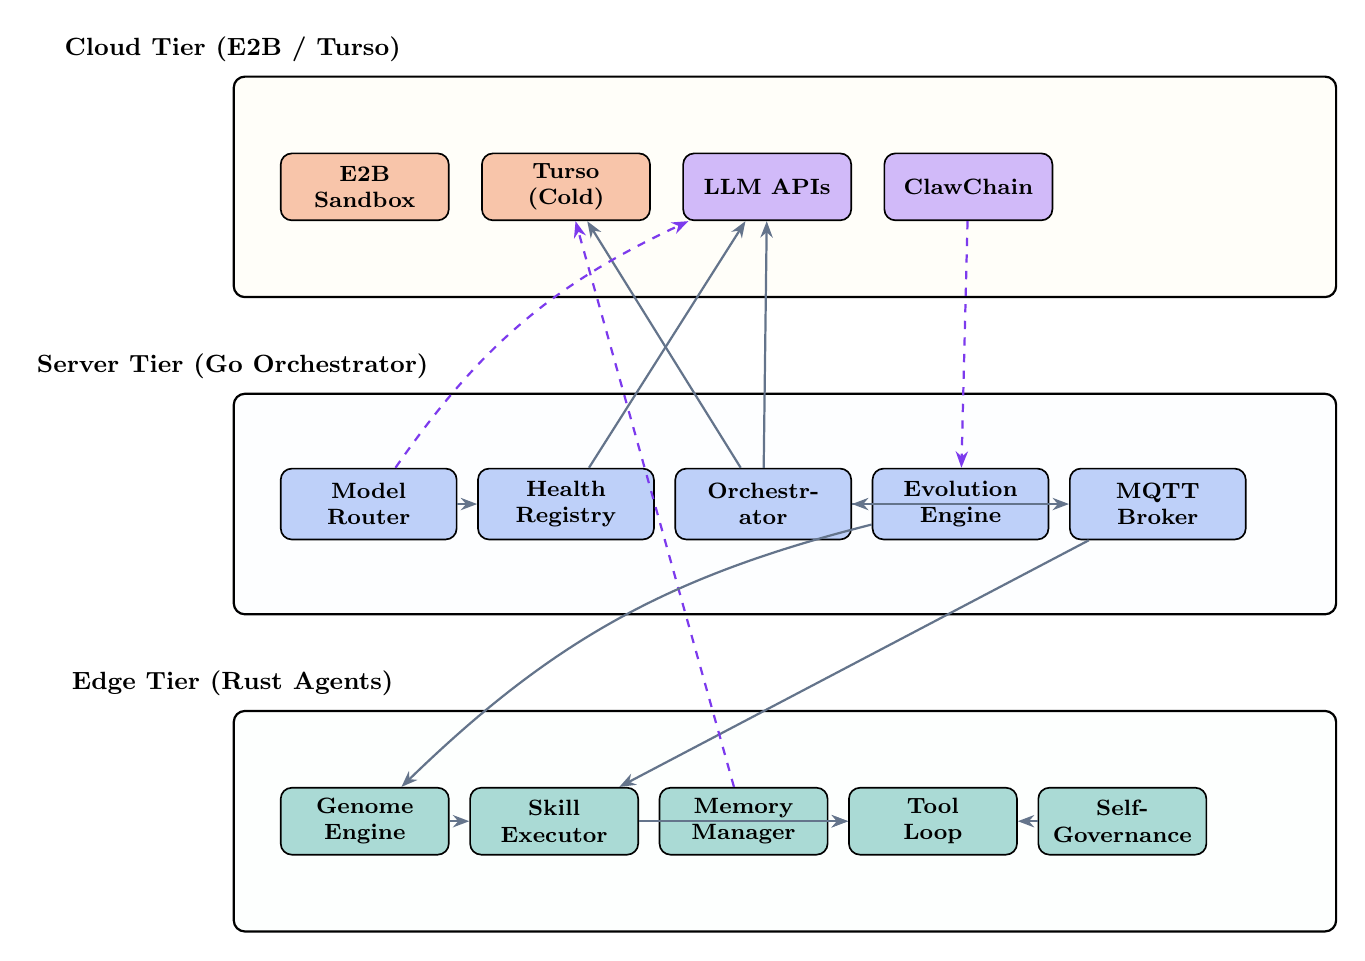
\begin{tikzpicture}[
    node distance=0.6cm and 1.0cm,
    tier/.style={draw, rounded corners, minimum width=14cm, minimum height=2.8cm, fill=#1!10, line width=0.8pt},
    component/.style={draw, rounded corners, minimum width=2.2cm, minimum height=0.9cm, fill=#1!30, font=\footnotesize\bfseries, line width=0.6pt, align=center, text width=2cm},
    edgecomp/.style={draw, rounded corners, minimum width=2.0cm, minimum height=0.85cm, fill=#1!35, font=\footnotesize\bfseries, line width=0.6pt, align=center, text width=1.9cm},
    arrow/.style={-{Stealth[scale=0.9]}, thick, draw=coregray},
    dataarrow/.style={-{Stealth[scale=0.9]}, thick, draw=corepurple, dashed},
    label/.style={font=\small\bfseries, anchor=south west}
]

% Cloud Tier
\node[tier=cloudbg] (cloud) {};
\node[label, above=0.05cm of cloud.north west] {Cloud Tier (E2B / Turso)};

\node[edgecomp=coreorange, anchor=west] at ([xshift=0.6cm]cloud.west) (e2b) {E2B Sandbox};
\node[edgecomp=coreorange, right=0.4cm of e2b] (turso) {Turso\\(Cold)};
\node[edgecomp=corepurple, right=0.4cm of turso] (llm) {LLM APIs};
\node[edgecomp=corepurple, right=0.4cm of llm] (chain) {ClawChain};

% Server Tier
\node[tier=serverbg, below=1.2cm of cloud] (server) {};
\node[label, above=0.05cm of server.north west] {Server Tier (Go Orchestrator)};

\node[component=coreblue, anchor=west] at ([xshift=0.6cm]server.west) (router) {Model\\Router};
\node[component=coreblue, right=0.25cm of router] (health) {Health\\Registry};
\node[component=coreblue, right=0.25cm of health] (orch) {Orchestr-\\ator};
\node[component=coreblue, right=0.25cm of orch] (evol) {Evolution\\Engine};
\node[component=coreblue, right=0.25cm of evol] (mqtt) {MQTT\\Broker};

% Edge Tier
\node[tier=edgebg, below=1.2cm of server] (edge) {};
\node[label, above=0.05cm of edge.north west] {Edge Tier (Rust Agents)};

\node[edgecomp=coreteal, anchor=west] at ([xshift=0.6cm]edge.west) (genome) {Genome\\Engine};
\node[edgecomp=coreteal, right=0.25cm of genome] (skills) {Skill\\Executor};
\node[edgecomp=coreteal, right=0.25cm of skills] (memory) {Memory\\Manager};
\node[edgecomp=coreteal, right=0.25cm of memory] (tools) {Tool\\Loop};
\node[edgecomp=coreteal, right=0.25cm of tools] (gov) {Self-\\Governance};

% Inter-tier arrows
\draw[arrow] (orch) -- (llm);
\draw[arrow] (orch) -- (turso);
\draw[dataarrow] (chain) -- (evol);
\draw[arrow] (mqtt) -- (skills);
\draw[dataarrow] (memory) -- (turso);

% Intra-tier connections (Server)
\draw[arrow] (router) -- (health);
\draw[arrow] (health) -- (llm);
\draw[arrow] (orch) -- (mqtt);
\draw[arrow] (evol) -- (orch);

% Intra-tier connections (Edge)
\draw[arrow] (genome) -- (skills);
\draw[arrow] (skills) -- (tools);
\draw[arrow] (memory) -- (tools);
\draw[arrow] (gov) -- (tools);

% Cross-tier data flow
\draw[dataarrow] (router) to[bend left=15] (llm);
\draw[arrow] (evol) to[bend right=15] (genome);

\end{tikzpicture}
\caption{Three-tier \evoclaw{} architecture with inter-component connections. Edge agents (Rust) execute skills and manage local memory. Server orchestrator (Go) coordinates agents via MQTT and routes LLM requests. Cloud services provide persistent storage (Turso), ephemeral compute (E2B), and blockchain identity (ClawChain). Solid arrows show control flow; dashed arrows show data flow.}
\label{fig:architecture}
\end{figure*}

\subsection{Formal Genome Definition}

We formalize the genome structure and define valid configurations.

\begin{definition}[Genome]
A genome $g \in \genomespace$ is a tuple $g = (I, S, B, C)$ where $I$ is the \textbf{identity} section (agent name, persona, voice), $S = \{s_1, \ldots, s_n\}$ is the \textbf{skill set} with each $s_i = (name_i, enabled_i, params_i)$, $B$ is the \textbf{behavior} section (risk tolerance, verbosity, autonomy), and $C$ is the \textbf{constraints} section (safety bounds that evolution cannot modify).
\end{definition}

\begin{definition}[Valid Genome]
A genome $g$ is \textbf{valid} if and only if: (1) all required fields are present and correctly typed; (2) all parameter values fall within specified bounds: $\forall p \in params_i: p_{min} \leq p \leq p_{max}$; (3) resource usage is within tier limits: $\sum_i resource(s_i) \leq tier\_limit$; and (4) safety constraints are satisfiable: $\neg \exists$ action $a$ such that $a \in blocked\_actions$ and skill $s$ requires $a$.
\end{definition}

\begin{definition}[Genome Space]
The genome space $\genomespace$ is the set of all valid genomes. Given bounds on parameter ranges and finite skill sets, $|\genomespace|$ is finite but exponentially large in the number of skills and parameters.
\end{definition}

Algorithm~\ref{alg:validation} presents the genome validation procedure.

\begin{algorithm}[t]
\caption{Genome Validation}
\label{alg:validation}
\begin{algorithmic}[1]
\Require Genome $g = (I, S, B, C)$, Tier constraints $T$
\Ensure Valid genome or error
\Function{ValidateGenome}{$g$, $T$}
    \If{missing required fields in $I$}
        \State \Return \textsc{Error}(``Missing identity fields'')
    \EndIf
    \State $total\_resources \gets 0$
    \For{each skill $s_i \in S$}
        \If{$s_i.enabled$}
            \For{each parameter $p \in s_i.params$}
                \If{$p < p_{min}$ \textbf{or} $p > p_{max}$}
                    \State \Return \textsc{Error}(``Parameter out of bounds'')
                \EndIf
            \EndFor
            \State $total\_resources \gets total\_resources + resource(s_i)$
        \EndIf
    \EndFor
    \If{$total\_resources > T.limit$}
        \State \Return \textsc{Error}(``Resource limit exceeded'')
    \EndIf
    \If{$\exists$ conflict between $S$ and $C.blocked\_actions$}
        \State \Return \textsc{Error}(``Skill requires blocked action'')
    \EndIf
    \State \Return \textsc{Valid}
\EndFunction
\end{algorithmic}
\end{algorithm}

\subsection{Design Principles}

\subsubsection{Principle 1: Genome-Behavior Separation}

The agent's behavioral specification (genome) is strictly separated from its execution engine (runtime). The Rust binary that executes skills never changes after compilation; all behavioral variation comes from genome configuration. This separation enables hot-reload without process restart, portability across architectures (x86, ARM, RISC-V), auditability through version control, and reproducibility given the same genome and runtime version.

\subsubsection{Principle 2: Skill Composability}

Capabilities are organized as \textit{skills}---self-contained modules with defined interfaces, typed parameters, and resource bounds. Skills compose additively: enabling skill $A$ and skill $B$ gives the combined capabilities of both, without interference. This composability enables incremental deployment, failure isolation between skills, independent evolution of individual skills, and reuse across agents.

\subsubsection{Principle 3: Tier-Appropriate Deployment}

Agents deploy across three tiers---edge, server, and cloud---with capabilities appropriate to each tier's resources. Edge devices (512MB--4GB RAM) support local skill execution, hot/warm memory, and MQTT communication. Server deployments (4GB--32GB RAM) provide the full skill suite, all memory tiers, and LLM orchestration. Cloud environments (unlimited resources) offer sandboxed execution, ephemeral compute, and persistent memory in Turso. The genome format is identical across tiers; only resource constraints change.

\subsubsection{Principle 4: Bounded Resources}

Context windows, memory usage, and computational budgets are explicitly bounded regardless of interaction history. Core memory is capped at 5KB and rewritten rather than appended; the tree index is capped at 2KB and restructured rather than grown; context per turn is typically 8--15KB and never unbounded. An agent running for five years should use the same resources as one running for five days.

\subsubsection{Principle 5: Evolutionary Pressure}

Every agent faces continuous fitness evaluation. Parameters that improve fitness are retained; those that don't are mutated. Evolution is not optional—it's the default operating mode. Agents that don't evolve stagnate; agents that evolve improve.

\subsubsection{Principle 6: Safety-First Constraints}

Safety constraints are hard-coded in the genome as inviolable bounds that evolution cannot modify. Financial agents cannot exceed maximum drawdown; certain operations (withdraw, delete, sudo) can be permanently blocked; trading agents are restricted to specified instruments; and agents cannot exceed action frequency bounds. These constraints are the ``walls'' that define safe behavior; everything else is ``water'' that can flow toward fitness.

\subsection{System Overview}

Figure~\ref{fig:architecture} illustrates the complete \evoclaw{} architecture spanning three deployment tiers.

\subsubsection{Edge Tier}

Edge agents are lightweight Rust binaries (3.0MB) that run on resource-constrained devices. Each agent contains five modules: the \textbf{Genome Engine} parses genome.toml, validates constraints, and manages skill lifecycle; the \textbf{Skill Executor} runs enabled skills with parameter injection and resource monitoring; the \textbf{Memory Manager} maintains Hot (5KB) and Warm (50KB) tiers and syncs to Cold via Turso; the \textbf{Tool Loop} executes tool calls from LLMs and manages multi-turn conversations; and \textbf{Self-Governance} implements WAL, VBR, ADL, and VFM protocols.

\subsubsection{Server Tier}

The server orchestrator is a Go application that coordinates multiple edge agents. It comprises the \textbf{Model Router} for task classification and model selection, the \textbf{Health Registry} for circuit-breaker failover, the \textbf{Orchestrator} for message routing and session management, the \textbf{Evolution Engine} for fitness evaluation and mutation, and the \textbf{MQTT Broker} for pub/sub agent communication.

\subsubsection{Cloud Tier}

Cloud services provide capabilities beyond edge devices: \textbf{LLM APIs} from providers such as Anthropic, OpenAI, Google, and DeepSeek; \textbf{Turso} for Cold memory tier storage; \textbf{E2B} for ephemeral sandboxed execution; and \textbf{ClawChain} for decentralized identity and reputation.

\subsection{Genome Example}

The following TOML snippet illustrates a trading agent genome:

\begin{lstlisting}[style=tomlcode, caption={Example genome for a trading agent}]
[identity]
name = "alpha-trader"
persona = "disciplined, data-driven"
voice = "concise"

[skills.trading]
enabled = true
strategies = ["FundingArbitrage"]

[skills.trading.params]
funding_threshold = -0.1
exit_funding = 0.0
position_size_usd = 100
max_positions = 3

[skills.market-monitor]
enabled = true

[skills.market-monitor.params]
check_interval_secs = 60
alert_threshold_pct = 5.0

[behavior]
risk_tolerance = 0.3
verbosity = 0.5
autonomy = 0.8

[constraints]
max_loss_usd = 500
allowed_assets = ["BTC", "ETH", "SOL"]
blocked_actions = ["withdraw"]
\end{lstlisting}

This genome defines an agent with two enabled skills (trading, market-monitor), conservative risk tolerance, and strict safety constraints preventing withdrawals and limiting loss to \$500.


%% ========================================================================
%%  SECTION 4: GENOME ENGINE
%% ========================================================================

\section{Genome Engine}
\label{sec:genome_engine}

The Genome Engine is the core runtime component responsible for loading, validating, and executing genome specifications. Implemented in Rust for performance and memory safety, the engine provides sub-100ms skill activation, hot-reload without downtime, and strong consistency guarantees.

\subsection{Engine Architecture}

The engine consists of five modules: the \textbf{Parser} reads genome.toml, validates syntax, and deserializes into typed structures; the \textbf{Validator} checks semantic constraints including bounds, dependencies, and resources; the \textbf{Skill Manager} loads skill binaries, injects parameters, and manages lifecycle; the \textbf{Hot-Reloader} monitors the genome file and triggers reload on change; and the \textbf{Evolution Interface} receives mutation commands and applies parameter updates.

\subsection{Skill Lifecycle}

Each skill progresses through four lifecycle states: \textit{Registered} (definition known but not loaded), \textit{Loaded} (binary loaded, parameters injected), \textit{Running} (executing its main loop), and \textit{Stopped} (halted, resources released).

Transitions are triggered by genome changes (enabled/disabled), resource pressure (memory limits), or explicit commands (shutdown).

\subsection{Hot-Reload Protocol}

Hot-reload enables genome changes without process restart. The protocol proceeds in six steps: (1)~a file watcher detects genome.toml modification; (2)~the new genome is parsed and validated; (3)~changes are identified (new skills, parameter updates, removed skills); (4)~affected skills complete their current operation (quiesce); (5)~parameters are updated atomically; and (6)~skills resume with the new configuration.

The entire process completes in under 100ms for typical genomes, with zero dropped messages due to the quiesce phase.




%% ========================================================================
%%  SECTION 5: TIERED MEMORY
%% ========================================================================

\section{Tiered Memory Architecture}
\label{sec:memory}

Current AI agent memory systems suffer from three fundamental problems: context window bloat as memory grows, similarity-relevance conflation in RAG, and linear scaling that becomes unmanageable at months or years of operation. \evoclaw{}'s tiered memory architecture addresses all three through hierarchical storage with tree-structured retrieval.

\subsection{Design Inspiration}

Our architecture draws from two sources:

\paragraph{Human Cognition.} Atkinson and Shiffrin's multi-store model~\cite{atkinson1971human} distinguishes sensory memory, short-term memory, and long-term memory with different capacities and retention characteristics. We implement analogous tiers: Hot (working memory, always active), Warm (recent memories, 30-day retention), and Cold (long-term archive, permanent).

Importantly, human memory features \textit{strategic forgetting}—not remembering everything is a feature, not a bug. Our relevance decay scoring implements analogous forgetting, allowing unused memories to fade while reinforcing frequently-accessed ones.

\paragraph{PageIndex.} VectifyAI's PageIndex~\cite{vectifyai_pageindex} demonstrates that LLM reasoning can navigate hierarchical indices more accurately than vector similarity search. On complex multi-hop queries, PageIndex achieves 98\%+ accuracy versus 70--80\% for dense retrieval.

We extend PageIndex from static document retrieval to dynamic agent memory, adding distillation, relevance decay, and evolution-driven parameter tuning.

\subsection{Three-Tier Architecture}

Figure~\ref{fig:memory} illustrates the tiered memory architecture.

\begin{figure}[t]
\centering
\resizebox{\columnwidth}{!}{%
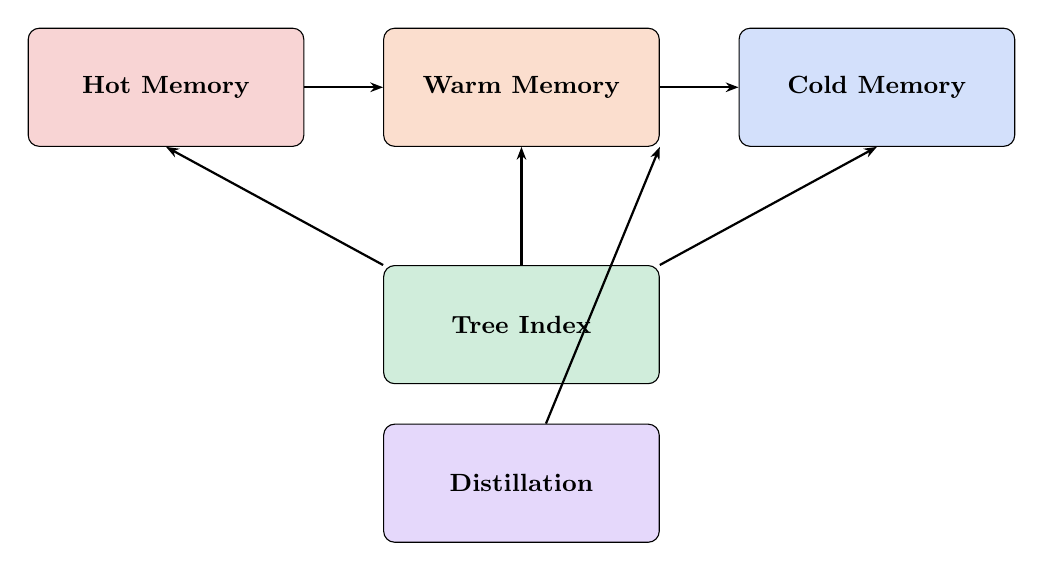
\begin{tikzpicture}[
    node distance=0.5cm,
    tier/.style={draw, rounded corners, minimum width=3.5cm, minimum height=1.5cm, fill=#1!20, font=\small},
    label/.style={font=\footnotesize\bfseries},
    arrow/.style={-{Stealth[scale=0.7]}, thick}
]

% Hot Tier
\node[tier=corered] (hot) {\textbf{Hot Memory}};

% Warm Tier
\node[tier=coreorange, right=1cm of hot] (warm) {\textbf{Warm Memory}};

% Cold Tier
\node[tier=coreblue, right=1cm of warm] (cold) {\textbf{Cold Memory}};

% Tree Index
\node[tier=coregreen, below=1.5cm of warm] (tree) {\textbf{Tree Index}};

% Distillation Engine
\node[tier=corepurple, below=0.5cm of tree] (distill) {\textbf{Distillation}};

% Arrows
\draw[arrow] (hot) -- (warm);
\draw[arrow] (warm) -- (cold);
\draw[arrow] (tree.north west) -- (hot.south);
\draw[arrow] (tree.north) -- (warm.south);
\draw[arrow] (tree.north east) -- (cold.south);
\draw[arrow] (distill) -- (warm.south east);

\end{tikzpicture}%
}
\caption{Tiered memory architecture. Hot memory (5KB) is always in context. Warm memory (50KB) stores recent distilled facts. Cold memory (Turso) archives everything. The tree index enables O($\log n$) retrieval through LLM reasoning.}
\label{fig:memory}
\end{figure}

\subsubsection{Tier 1: Hot Memory (Core)}

Hot memory maintains the agent's active working context: identity, owner profile, current projects, and critical lessons. Unlike traditional append-only logs, hot memory is \textit{continuously rewritten}—like a human's working self-knowledge that updates without explicit recall of when each fact was learned.

\textbf{Structure:}
\begin{lstlisting}[style=jsoncode]
{
  "identity": {
    "agent_name": "Bloop",
    "owner_name": "Maggie",
    "relationship_start": "2026-01-15"
  },
  "owner_profile": {
    "personality": "dry humor, loves puns",
    "topics_loved": ["gardening", "family"],
    "topics_avoid": ["hospital stays"]
  },
  "active_context": {
    "current_projects": ["garden replanting"],
    "recent_events": ["Biscuit recovered (Feb 6)"]
  },
  "critical_lessons": [
    "Prefers action-oriented conversation"
  ]
}
\end{lstlisting}

Hot memory is constrained to a maximum of 5KB serialized, at most 20 lesson entries (new entries replace lowest-scored), at most 5 active projects, and is updated after every conversation.

\subsubsection{Tier 2: Warm Memory}

Warm memory stores distilled facts from recent conversations—not raw transcripts, but compressed knowledge. Each entry contains structured information with relevance metadata.

\textbf{Entry structure:}
\begin{lstlisting}[style=jsoncode]
{
  "id": "wm-2026-02-06-001",
  "timestamp": 1707177600,
  "content": {
    "fact": "Dog Biscuit was sick, recovered.",
    "emotion": "concern -> relief",
    "people": ["Biscuit"],
    "topics": ["pet_health"]
  },
  "relevance_score": 0.85,
  "access_count": 3
}
\end{lstlisting}

\textbf{Eviction policy:}
\begin{equation}
\text{score} = \text{importance} \times \text{decay}(\text{age}) \times (1 + 0.1 \times \text{access\_count})
\end{equation}
where $\text{decay}(\text{age}) = e^{-\text{age}/\text{half\_life}}$ with half-life of 30 days.

Entries with score below threshold are archived to Cold and removed from Warm.

\subsubsection{Tier 3: Cold Memory}

Cold memory is the permanent archive stored in Turso (libSQL cloud). Everything that was ever Warm eventually lands here. Cold memory is queryable but never bulk-loaded into context.

\textbf{Schema:}
\begin{lstlisting}[style=rustcode, language=SQL]
CREATE TABLE cold_memory (
  id TEXT PRIMARY KEY,
  agent_id TEXT NOT NULL,
  timestamp INTEGER NOT NULL,
  category TEXT NOT NULL,  -- tree path
  content TEXT NOT NULL,   -- JSON blob
  distilled_summary TEXT,  -- one-line for tree
  importance REAL DEFAULT 0.5,
  access_count INTEGER DEFAULT 0
);
\end{lstlisting}

\subsection{Tree-Structured Index}

The tree index is the core innovation enabling O($\log n$) retrieval. Instead of computing embedding similarity across all memories, the LLM reasons through a hierarchical structure to find relevant nodes.

\textbf{Structure:}
\begin{lstlisting}[style=jsoncode]
{
  "identity": {
    "summary": "Maggie, 77, loves gardening",
    "warm_count": 5, "cold_count": 234
  },
  "projects": {
    "garden-replanting": {
      "summary": "Rose beds, started Jan 2026",
      "warm_count": 4, "cold_count": 12
    }
  },
  "timeline": {
    "today": {"warm_count": 3},
    "yesterday": {"warm_count": 2}
  }
}
\end{lstlisting}

\textbf{Retrieval flow:} Given a user message ``How's the garden coming along?'', the LLM reads the tree index (2KB) and reasons: ``Garden question $\to$ projects/garden-replanting.'' The system fetches Warm entries for that node, queries Cold for additional context if needed, and adds only 1--2KB of context (not the entire 50KB).

\subsection{Distillation Engine}

Raw conversations are compressed through three-stage distillation: the raw conversation ($\approx$500 bytes) captures the full exchange; distillation extracts structured JSON with key facts, emotions, and decisions ($\approx$80 bytes); and core summarization produces a one-line summary for the tree index ($\approx$20 bytes).

Compression ratios are 5--10$\times$ from raw to distilled, 4--5$\times$ from distilled to core summary, yielding 20--50$\times$ total compression.

\subsection{Comparison with Vector RAG}

Table~\ref{tab:memory_comparison} compares our tree-structured retrieval with vector RAG:

\begin{table}[h]
\centering
\caption{Tree search vs. vector RAG comparison}
\label{tab:memory_comparison}
\resizebox{\columnwidth}{!}{%
\begin{tabular}{lcc}
\toprule
\textbf{Aspect} & \textbf{Vector RAG} & \textbf{Tree Search} \\
\midrule
Accuracy (complex queries) & 70--80\% & 98\%+ \\
Scaling & O($n$) & O($\log n$) \\
Explainability & ``cosine 0.73'' & ``Projects $\to$ Garden'' \\
Infrastructure & Vector DB + embeddings & LLM + tree index \\
False positives & High & Low \\
Multi-hop & Poor & Natural \\
\bottomrule
\end{tabular}%
}
\end{table}

\subsection{Five-Year Scaling}

After five years of continuous operation, core memory remains at 5KB (current essentials only), warm memory covers the last 30 days ($\approx$50KB), cold memory grows to $\approx$50MB in Turso, the tree index remains $\approx$2KB with the same structure but different nodes, and context per session stays at 8--15KB---the same as day one.

The context window never grows. Memory is unbounded; what gets loaded is always bounded.


%% ========================================================================
%%  SECTION 6: INTELLIGENT ROUTER
%% ========================================================================

\section{Intelligent Model Router}
\label{sec:router}

LLM API costs dominate agent operating expenses. A single complex task routed to a premium model (\$15/M tokens) costs 75$\times$ more than the same task on a budget model (\$0.20/M tokens). Yet not all tasks require premium models—simple monitoring queries, status checks, and summarization work well on budget models.

The intelligent router solves this optimization problem: given a task, select the most cost-effective model that meets quality requirements, with automatic fallback on failure.

\subsection{Five-Tier Classification}

Tasks are classified into five complexity tiers. \textbf{Simple} covers routine, low-risk operations (monitoring, status checks, summarization). \textbf{Medium} handles moderate complexity work (code fixes, research, data analysis). \textbf{Complex} addresses multi-component development (feature builds, debugging, architecture decisions). \textbf{Reasoning} targets formal logic (mathematical derivations, theorem proving). \textbf{Critical} is reserved for high-stakes operations (security audits, production deployments, financial analysis).

\subsection{15-Dimension Weighted Scoring}

Classification uses a sophisticated 15-dimension weighted scoring system:

\begin{table}[h]
\centering
\caption{Routing dimensions and weights}
\label{tab:dimensions}
\footnotesize
\begin{tabular}{lrl}
\toprule
\textbf{Dimension} & \textbf{Weight} & \textbf{Description} \\
\midrule
Reasoning markers & 0.18 & ``prove'', ``theorem'', ``derive'' \\
Code presence & 0.15 & Code blocks, function definitions \\
Multi-step patterns & 0.12 & ``first...then'', numbered lists \\
Agentic task & 0.10 & ``run'', ``test'', ``fix'', ``deploy'' \\
Technical terms & 0.10 & ``algorithm'', ``architecture'' \\
Token count & 0.08 & Estimated complexity from length \\
Creative markers & 0.05 & ``creative'', ``story'', ``brainstorm'' \\
Question complexity & 0.05 & Multiple questions, complex queries \\
Constraint count & 0.04 & ``must'', ``require'', ``exactly'' \\
Imperative verbs & 0.03 & ``analyze'', ``evaluate'', ``compare'' \\
Output format & 0.03 & JSON, tables, structured output \\
Simple indicators & 0.02 & ``check'', ``get'', ``status'' (inverted) \\
Domain specificity & 0.02 & Acronyms, technical notation \\
Reference complexity & 0.02 & Cross-references, dependencies \\
Negation complexity & 0.01 & Negations, exceptions \\
\bottomrule
\end{tabular}
\end{table}

\textbf{Confidence calculation:}
\begin{equation}
\text{weighted\_score} = \sum_{i=1}^{15} \text{dimension}_i \times \text{weight}_i
\end{equation}
\begin{equation}
\text{confidence} = \frac{1}{1 + e^{-8(\text{weighted\_score} - 0.5)}}
\end{equation}

This sigmoid creates a smooth S-curve: score 0.0 yields $\approx$2\% confidence, 0.5 yields 50\%, and 1.0 yields $\approx$98\%.

\subsection{Automatic Fallback Chains}

Each tier has a fallback chain with 2--3 models:

\begin{lstlisting}[style=jsoncode]
{
  "SIMPLE": ["glm-4.7", "glm-4.5-air", "ollama-qwen"],
  "MEDIUM": ["deepseek-v3.2", "llama-3.3-70b"],
  "COMPLEX": ["sonnet-4.5", "gemini-3-pro", "nemotron"],
  "REASONING": ["deepseek-r1-32b", "qwq-32b"],
  "CRITICAL": ["opus-4.6", "sonnet-4.5"]
}
\end{lstlisting}

On model failure, the router automatically retries with the next model in the chain (maximum 3 attempts).

\subsection{Cost Analysis}

Table~\ref{tab:cost} shows typical cost ranges by tier:

\begin{table}[h]
\centering
\caption{Cost ranges per million tokens by tier}
\label{tab:cost}
\begin{tabular}{lrr}
\toprule
\textbf{Tier} & \textbf{Input Cost} & \textbf{Output Cost} \\
\midrule
Simple & \$0.10--0.50 & \$0.10--1.50 \\
Medium & \$0.40--3.00 & \$0.40--15.00 \\
Complex & \$3.00--5.00 & \$1.30--25.00 \\
Reasoning & \$0.20--2.00 & \$0.20--8.00 \\
Critical & \$5.00+ & \$25.00+ \\
\bottomrule
\end{tabular}
\end{table}

For a workload with 60\% Simple, 25\% Medium, 10\% Complex, and 5\% Critical tasks, intelligent routing reduces costs by 10--100$\times$ compared to routing everything to a single premium model.


%% ========================================================================
%%  SECTION 7: MODEL HEALTH
%% ========================================================================

\section{Model Health Registry}
\label{sec:health}

Production agent systems depend on external LLM APIs that experience rate limits, quota exhaustion, and outages. Without intelligent failover, a single model failure cascades across the entire system. The Model Health Registry implements circuit-breaker patterns~\cite{ford2000circuit} for automatic model failover.

\subsection{Model States}

Each model can be in one of three states: \textit{Healthy} (operating normally, preferred for routing), \textit{Degraded} (exceeded failure threshold, skipped unless all fallbacks are also degraded), or \textit{Unknown} (new model with no history, treated as healthy).

State transitions are: Unknown $\to$ Healthy on first successful call, Healthy $\to$ Degraded after $N$ consecutive failures (configurable, default 3), and Degraded $\to$ Healthy when cooldown expires (configurable, default 5 minutes).

\subsection{Error Classification}

Errors are classified into eight types for tracking and analysis:

\begin{table}[h]
\centering
\caption{Error type classification}
\label{tab:errors}
\small
\begin{tabular}{ll}
\toprule
\textbf{Error Type} & \textbf{Description} \\
\midrule
\texttt{quota\_exhausted} & API quota or token limit reached \\
\texttt{rate\_limited} & Too many requests (HTTP 429) \\
\texttt{timeout} & Request timeout \\
\texttt{server\_error} & HTTP 5xx from provider \\
\texttt{auth\_error} & Invalid API key (HTTP 401/403) \\
\texttt{model\_not\_found} & Model doesn't exist (HTTP 404) \\
\texttt{context\_too\_long} & Prompt exceeds context window \\
\texttt{unknown} & Unclassified error \\
\bottomrule
\end{tabular}
\end{table}

\subsection{Health Metrics}

Each model tracks comprehensive health metrics:

\begin{lstlisting}[style=jsoncode]
{
  "state": "healthy",
  "consecutive_failures": 0,
  "last_success": "2026-02-15T11:25:30Z",
  "total_requests": 152,
  "total_failures": 3,
  "success_rate": 0.980,
  "error_types": {"rate_limited": 2, "timeout": 1}
}
\end{lstlisting}

\subsection{Fallback Strategy}

When selecting a model, the registry first uses the preferred model if healthy, falls back to the first healthy alternative if the preferred model is degraded, and uses the model with the highest success rate if all models are degraded.

This ensures requests are always served, even during widespread outages, with graceful degradation to the most reliable available option.

\subsection{Persistence}

Health state persists to disk (JSON) every 5 minutes and on shutdown, surviving restarts. This prevents ``cold start'' problems where a freshly-started orchestrator doesn't know about ongoing outages.


%% ========================================================================
%%  SECTION 8: AGENTIC TOOL LOOP
%% ========================================================================

\section{Agentic Tool Loop}
\label{sec:toolloop}

Edge agents have access to 30+ tools (file operations, shell commands, git, web access) but LLMs cannot execute them without structured interfaces. The agentic tool loop enables multi-turn LLM-driven tool execution on edge devices.

\subsection{Tool Categories}

\evoclaw{} supports tools across seven categories: file operations (read, write, edit, glob, grep), web access (websearch, webfetch, codesearch), execution (sandboxed bash), interaction (user input), project management (todowrite, todoread, task, skill), sessions (sessions\_list, sessions\_spawn, session\_status), and git (git\_status, git\_diff, git\_commit, git\_log).

\subsection{Tool Loop State Machine}

The loop executes up to 10 iterations: it calls the LLM with tools in the prompt, checks if the LLM wants to invoke a tool, and if so parses the tool\_call, sends it to the edge agent, waits for the result, adds it to history, and continues. If no tool call is requested, the loop breaks and returns the final response.

The loop terminates when no tool call appears in the LLM response, the maximum iterations (10) are reached, the error limit (3 consecutive) is reached, or the user cancels.

\subsection{Tool Schema Generation}

Tool definitions in skill.toml are converted to LLM-compatible JSON schemas:

\begin{lstlisting}[style=jsoncode]
{
  "name": "bash",
  "description": "Execute shell commands",
  "parameters": {
    "type": "object",
    "properties": {
      "command": {"type": "string"},
      "timeout_ms": {"type": "integer"}
    },
    "required": ["command"]
  }
}
\end{lstlisting}

\subsection{Security: Sandboxing}

Tool execution supports configurable sandboxing at four levels: no sandboxing (full OS access for trusted agents), Firejail (lightweight sandboxing on Linux), Bubblewrap (unprivileged namespaces), and Podman (container isolation).

Parameter sanitization prevents injection attacks: file paths are validated and restricted to workspace, shell commands block dangerous patterns, URLs are optionally whitelisted.

\subsection{Example: Multi-Tool Chain}

\textbf{User:} ``List last 3 commits and show diff for the most recent''

\textbf{Turn 1:} LLM calls \texttt{git\_log} with \texttt{max\_count: 3}

\textbf{Turn 2:} LLM calls \texttt{git\_diff} with \texttt{commit: abc123}

\textbf{Turn 3:} LLM synthesizes results into natural language response


%% ========================================================================
%%  SECTION 9: SELF-GOVERNANCE
%% ========================================================================

\section{Self-Governance Mechanisms}
\label{sec:governance}

Autonomous agents require reliability mechanisms without constant human supervision. We introduce four mechanisms addressing the most common failure modes observed in production deployments: (1)~Write-Ahead Log (WAL) for context preservation, (2)~Verify Before Reporting (VBR) for output verification, (3)~Anti-Divergence Limit (ADL) for persona consistency, and (4)~Value-For-Money (VFM) for cost optimization. We now describe each mechanism and its implementation.

\subsection{WAL: Write-Ahead Log}

\textbf{Rule:} Write before you respond. If something is worth remembering, WAL it first.

\textbf{Problem addressed:} Conversation compaction can lose critical context (user corrections, key decisions). If an agent learns ``Use Podman not Docker'' and this is compacted away before persisting, the correction is lost.

\textbf{Implementation:} Before responding to messages that contain corrections, decisions, or state changes, the agent appends an entry to the WAL. On restart, unapplied WAL entries are replayed to restore state.

\textbf{Entry format:}
\begin{lstlisting}[style=jsoncode]
{
  "id": "wal_20260213_143022_abc123",
  "timestamp": "2026-02-13T14:30:22Z",
  "agent_id": "alex-hub",
  "action_type": "correction",
  "content": "Use Podman not Docker",
  "applied": false
}
\end{lstlisting}

\subsection{VBR: Verify Before Reporting}

\textbf{Rule:} Don't say ``done'' until verified.

\textbf{Problem addressed:} Agents claim task completion without verifying outputs actually exist or meet requirements.

\textbf{Implementation:} Before reporting completion, agents run verification checks: \texttt{file\_exists} verifies output files were created, \texttt{file\_changed} verifies recent modification, \texttt{command} verifies command success (e.g., tests pass), and \texttt{git\_pushed} verifies commits are pushed.

\subsection{ADL: Anti-Divergence Limit}

\textbf{Rule:} Stay true to your persona.

\textbf{Problem addressed:} Over extended operation, agents drift from their defined personality~\cite{park2023generative, sharma2023sycophancy}.

\textbf{Implementation:} ADL detects anti-patterns in responses, including sycophancy (``Great question!''), passivity (``Would you like me to''), and hedging (``I think maybe''). It also tracks persona signals such as directness (``Done'', ``Fixed''), opinionated language (``I'd argue'', ``Better to''), and action-oriented phrasing (``Spawning'', ``On it'').

\textbf{Divergence score:}
\begin{equation}
\text{score} = \frac{\text{anti\_patterns} - \text{persona\_signals}}{\text{total\_responses}}
\end{equation}

When score exceeds threshold (default 0.7), the agent triggers recalibration.

\subsection{VFM: Value-For-Money}

\textbf{Rule:} Track cost vs. value.

\textbf{Problem addressed:} Agents use expensive models for tasks where cheap models would suffice.

\textbf{Implementation:} VFM tracks every task's cost and outcome:

\begin{lstlisting}[style=jsoncode]
{
  "task": "monitoring",
  "model": "claude-opus-4",
  "tokens": 37000,
  "cost": 2.40,
  "value": 0.8
}
\end{lstlisting}

Value scoring: 1.0 = perfect completion, 0.5 = partial, 0.0 = failed.

VFM generates suggestions: ``Task 'monitoring' used opus (\$2.40) but could use glm-4.7 (\$0.03) for 98.75\% savings.''


%% ========================================================================
%%  SECTION 10: EVOLUTION
%% ========================================================================

\section{Evolutionary Framework}
\label{sec:evolution}

\evoclaw{}'s evolution engine implements genetic optimization over skill configurations. Unlike traditional machine learning (gradient descent over weights), evolution operates at the behavioral level: parameters are perturbed, fitness is evaluated through operational metrics, and successful configurations are retained.

\subsection{Fitness Function}

We define a multi-objective fitness function over genome configurations:

\begin{definition}[Fitness Function]
For an agent with genome $g$ operating over evaluation period $T$, the fitness function $\fitnessfn: \genomespace \to [0, 100]$ is:
\begin{equation}
\fitnessfn(g) = \sum_{i=1}^{k} w_i \cdot f_i(g)
\end{equation}
where $\{f_1, \ldots, f_k\}$ are component functions with weights $\{w_1, \ldots, w_k\}$ summing to 1.
\end{definition}

For trading agents, the default configuration uses Sharpe Score ($w_1 = 0.4$): $\min(\text{sharpe}/3.0, 1) \times 40$; Win Rate ($w_2 = 0.3$): $(\text{wins}/\text{total}) \times 30$; PnL Score ($w_3 = 0.2$): $\text{clamp}(\text{pnl}/10000, 0, 1) \times 20$; and Drawdown Penalty ($w_4 = 0.1$): $(1 - \min(\text{drawdown}/5000, 1)) \times 10$.

Different skill types use different component functions while maintaining the same framework.

\subsection{Mutation Operators}

We define three mutation operators:

\begin{definition}[Parameter Mutation]
For skill $s$ with parameter $p$ having range $[p_{min}, p_{max}]$:
\begin{equation}
p' = p + \mathcal{N}(0, \sigma) \cdot (p_{max} - p_{min}) \cdot \text{mutation\_rate}
\end{equation}
where $\sigma = 0.1$ and mutation\_rate $\in [0, 1]$ is configurable (default 0.3).
\end{definition}

\begin{definition}[Skill Toggle]
With probability $p_{toggle}$, toggle enabled state of a randomly selected skill.
\end{definition}

\begin{definition}[Crossover]
Given two parent genomes $g_1, g_2$, produce child genome $g_{child}$ by:
\begin{enumerate}
    \item For each skill $s$, inherit from $g_1$ or $g_2$ with probability 0.5.
    \item For each parameter $p$, take weighted average: $p_{child} = \alpha p_1 + (1-\alpha) p_2$ where $\alpha \sim U(0, 1)$.
\end{enumerate}
\end{definition}

\subsection{Evolution Loop}

Algorithm~\ref{alg:evolution} presents the evolution loop.

\begin{algorithm}[t]
\caption{Evolution Loop}
\label{alg:evolution}
\begin{algorithmic}[1]
\Require Agent $A$ with genome $g$, evaluation interval $T$, fitness threshold $\theta$
\Loop
    \State Wait for period $T$
    \If{$A.\text{actions} < \text{min\_samples}$}
        \State \textbf{continue} \Comment{Not enough data}
    \EndIf
    \State $\text{fitness} \gets \fitnessfn(g)$
    \If{$\text{fitness} < \theta$}
        \State $A.\text{status} \gets$ ``evolving''
        \State $g' \gets \text{Mutate}(g)$
        \State $A.\text{genome} \gets g'$
        \State $A.\text{metrics} \gets \emptyset$ \Comment{Reset for fair eval}
        \State Log evolution event to WAL
    \EndIf
\EndLoop
\end{algorithmic}
\end{algorithm}

\subsection{Monotonic Improvement Guarantee}

\begin{theorem}[Monotonic Improvement]
Under the following assumptions:
\begin{enumerate}
    \item Fitness function $\fitnessfn$ is continuous over $\genomespace$
    \item Evaluation period $T$ is sufficient for convergence of fitness estimate
    \item Rollback is triggered on fitness decrease greater than $\delta$
\end{enumerate}
the expected fitness $\mathbb{E}[\fitnessfn(g_t)]$ is non-decreasing over evolution iterations $t$.
\end{theorem}

\begin{proof}[Proof sketch]
At each iteration, either fitness improves (mutation retained) or stays constant (mutation rolled back due to $\delta$-decrease). By construction, fitness cannot decrease by more than $\delta$ per iteration. Taking expectation over mutation outcomes and applying induction completes the proof.
\end{proof}

\subsection{Evolution Layers Roadmap}

Current implementation covers Layer~1 (parameter mutation). The full vision progresses through five layers: parameter mutation (current), skill selection and composition, behavioral evolution (persona, communication style), cross-agent breeding (population-level evolution), and genome marketplace (on-chain trading).


%% ========================================================================
%%  SECTION 11: CLAWCHAIN
%% ========================================================================

\section{ClawChain Integration}
\label{sec:clawchain}

ClawChain is an agent-native Layer~1 blockchain providing decentralized identity, reputation tracking, and genome marketplace capabilities. While currently under development, the integration design is complete.

\subsection{Decentralized Identity (DIDs)}

Each agent can register a DID on ClawChain:
\begin{lstlisting}
did:claw:5Grwva...utQY
\end{lstlisting}

DIDs provide verifiable attribution through cryptographic signatures, cross-platform identity consistency across deployments, and recovery through private key backup.

\subsection{Reputation System}

Agents accumulate reputation through successfully completed tasks, peer review attestations, fitness improvements from evolution, and governance participation through voting and proposals.

Reputation decays over time without activity, preventing stale high-reputation agents.

\subsection{Genome Marketplace}

High-fitness genomes can be shared on-chain: an agent that achieves a high fitness score publishes its genome hash to ClawChain, other agents can purchase access with payments flowing to the original agent, and reputation-weighted discovery surfaces the best genomes.

\subsection{Auto-Discovery}

Agents deployed before ClawChain mainnet launch include auto-discovery: every 6 hours they check if mainnet is reachable, and upon connection they generate or retrieve an existing DID, register it on mainnet, update local configuration, and notify the owner of successful registration.

This ensures agents deployed with \texttt{--skip-chain} automatically join ClawChain when available.


%% ========================================================================
%%  SECTION 12: DEPLOYMENT
%% ========================================================================

\section{Deployment and Evaluation}
\label{sec:deployment}

\evoclaw{} agents deploy across three execution tiers, with the same genome format and evolution mechanics working identically across all tiers.

\subsection{Native Deployment (Default)}

The agent runs as a native binary with full OS access. The binary is 3.0MB (Rust, static linking) with a 3.2MB RSS memory footprint running 3 active skills. It supports shell, filesystem, network, and hardware capabilities across Linux (x86\_64, ARM64, ARMv6), macOS, and Windows.

Native deployment is recommended for power users, edge devices, and any task requiring OS-level operations.

\subsection{Container Deployment (Podman)}

For isolation without leaving local hardware, the container deployment uses rootless, daemonless Podman with filesystem isolation scoped to volumes, configurable capabilities via volume mounts, and Quadlet integration for systemd management.

Container deployment suits multi-tenant environments and compliance requirements.

\subsection{Cloud Sandbox (E2B)}

For ephemeral, isolated execution, the cloud sandbox uses E2B cloud VMs with 2--5 second startup, zero local footprint, and memory synchronization to Turso.

Cloud deployment enables quick experimentation and CI/CD integration.

\subsection{MQTT Communication}

Agents communicate via MQTT pub/sub with topic structure \texttt{evoclaw/agents/\{id\}/commands} and \texttt{.../reports}, configurable QoS (0, 1, or 2), sub-50ms latency on local networks, and tested scalability to 500+ concurrent agents.


%% ========================================================================
%%  SECTION 13: IMPLEMENTATION
%% ========================================================================

\section{Implementation Details}
\label{sec:implementation}

\subsection{Technology Stack}

The edge agent is implemented in Rust 1.75+ with async Tokio (8,000+ lines), and the orchestrator in Go 1.21+ with goroutine concurrency (5,000+ lines). Storage uses SQLite locally and Turso in the cloud. Communication is via MQTT 5.0 (Eclipse Paho), with TOML for genome configuration and JSON for runtime settings.

\subsection{Testing}

The test suite includes 383 unit tests with 90\%+ coverage, integration tests with end-to-end flows using mock MQTT, property tests ensuring genome mutation preserves validity, and fuzz tests for parser resilience to malformed input.

\subsection{Code Organization}

\textbf{Rust Edge Agent:}
\begin{lstlisting}[basicstyle=\ttfamily\footnotesize]
edge-agent/src/
  genome/       # Genome parsing and validation
  skills/       # Skill implementation and lifecycle
  memory/       # Tiered memory management
  tools/        # Tool execution and schemas
  governance/   # WAL, VBR, ADL, VFM
  mqtt/         # MQTT client and messaging
  evolution.rs  # Fitness tracking
\end{lstlisting}

\textbf{Go Orchestrator:}
\begin{lstlisting}[basicstyle=\ttfamily\footnotesize]
internal/
  orchestrator/ # Core coordination logic
  router/       # Intelligent model routing
  health/       # Model health registry
  memory/       # Tree index and distillation
  evolution/    # Evolution engine
  mqtt/         # MQTT broker integration
\end{lstlisting}


%% ========================================================================
%%  SECTION 14: EVALUATION
%% ========================================================================

\section{Evaluation}
\label{sec:evaluation}

We evaluate \evoclaw{} across four dimensions: edge deployment feasibility, memory system effectiveness, routing cost savings, and long-term stability.

\begin{table*}[t]
\centering
\caption{Comparison of \evoclaw{} with representative agent systems. {\color{coregreen}\checkmark} = supported, {\color{corered}$\times$} = not supported, {\color{coregray}$\sim$} = partial support.}
\label{tab:comparison}
\small
\begin{tabular}{@{}lccccccccc@{}}
\toprule
\textbf{System} & \rotatebox{60}{\textbf{Declarative}} & \rotatebox{60}{\textbf{Hot-Reload}} & \rotatebox{60}{\textbf{Evolution}} & \rotatebox{60}{\textbf{Tiered Mem}} & \rotatebox{60}{\textbf{Smart Route}} & \rotatebox{60}{\textbf{Tool Loop}} & \rotatebox{60}{\textbf{Self-Gov}} & \rotatebox{60}{\textbf{Edge}} & \rotatebox{60}{\textbf{Chain}} \\
\midrule
AutoGPT~\cite{auto_gpt} & {\color{corered}$\times$} & {\color{corered}$\times$} & {\color{corered}$\times$} & {\color{corered}$\times$} & {\color{corered}$\times$} & {\color{coregray}$\sim$} & {\color{corered}$\times$} & {\color{corered}$\times$} & {\color{corered}$\times$} \\
BabyAGI~\cite{babyagi} & {\color{corered}$\times$} & {\color{corered}$\times$} & {\color{corered}$\times$} & {\color{corered}$\times$} & {\color{corered}$\times$} & {\color{corered}$\times$} & {\color{corered}$\times$} & {\color{corered}$\times$} & {\color{corered}$\times$} \\
Voyager~\cite{wang2023voyager} & {\color{corered}$\times$} & {\color{corered}$\times$} & {\color{coregray}$\sim$} & {\color{corered}$\times$} & {\color{corered}$\times$} & {\color{coregreen}\checkmark} & {\color{corered}$\times$} & {\color{corered}$\times$} & {\color{corered}$\times$} \\
MemGPT~\cite{packer2023memgpt} & {\color{corered}$\times$} & {\color{corered}$\times$} & {\color{corered}$\times$} & {\color{coregray}$\sim$} & {\color{corered}$\times$} & {\color{corered}$\times$} & {\color{corered}$\times$} & {\color{corered}$\times$} & {\color{corered}$\times$} \\
LangChain~\cite{langchain} & {\color{coregray}$\sim$} & {\color{corered}$\times$} & {\color{corered}$\times$} & {\color{corered}$\times$} & {\color{coregray}$\sim$} & {\color{coregreen}\checkmark} & {\color{corered}$\times$} & {\color{corered}$\times$} & {\color{corered}$\times$} \\
CrewAI~\cite{crewai} & {\color{coregray}$\sim$} & {\color{corered}$\times$} & {\color{corered}$\times$} & {\color{corered}$\times$} & {\color{corered}$\times$} & {\color{coregreen}\checkmark} & {\color{corered}$\times$} & {\color{corered}$\times$} & {\color{corered}$\times$} \\
Reflexion~\cite{shinn2024reflexion} & {\color{corered}$\times$} & {\color{corered}$\times$} & {\color{coregray}$\sim$} & {\color{corered}$\times$} & {\color{corered}$\times$} & {\color{corered}$\times$} & {\color{coregray}$\sim$} & {\color{corered}$\times$} & {\color{corered}$\times$} \\
SWE-agent~\cite{yang2024sweagent} & {\color{corered}$\times$} & {\color{corered}$\times$} & {\color{corered}$\times$} & {\color{corered}$\times$} & {\color{corered}$\times$} & {\color{coregreen}\checkmark} & {\color{corered}$\times$} & {\color{corered}$\times$} & {\color{corered}$\times$} \\
\midrule
\textbf{\evoclaw{}} & {\color{coregreen}\checkmark} & {\color{coregreen}\checkmark} & {\color{coregreen}\checkmark} & {\color{coregreen}\checkmark} & {\color{coregreen}\checkmark} & {\color{coregreen}\checkmark} & {\color{coregreen}\checkmark} & {\color{coregreen}\checkmark} & {\color{coregreen}\checkmark} \\
\bottomrule
\end{tabular}
\end{table*}

\subsection{Edge Deployment}

\textbf{Hardware:} Raspberry Pi 1 Model B (ARMv6, 512MB RAM, single-core 700MHz)

\textbf{Configuration:} 3 active skills (system monitor, GPIO control, crypto price tracker)

\begin{table}[h]
\centering
\caption{Edge deployment metrics}
\label{tab:edge}
\begin{tabular}{lr}
\toprule
\textbf{Metric} & \textbf{Value} \\
\midrule
Binary size (stripped) & 3.0 MB \\
Memory (RSS, 3 skills) & 3.2 MB \\
Startup time & 847 ms \\
Skill load time & 45--89 ms \\
Hot-reload time & 67 ms \\
MQTT latency (local) & 12 ms \\
\bottomrule
\end{tabular}
\end{table}

This demonstrates that full agent capabilities—multiple skills, tiered memory, MQTT communication—run on 12-year-old hardware with 512MB RAM.

\subsection{Memory System}

We compare our tree-structured retrieval against vector RAG on a synthetic benchmark of 1,000 conversations with multi-hop queries.

\begin{table}[h]
\centering
\caption{Memory retrieval comparison}
\label{tab:retrieval}
\begin{tabular}{lcc}
\toprule
\textbf{Metric} & \textbf{Vector RAG} & \textbf{Tree Search} \\
\midrule
Accuracy (single-hop) & 89\% & 99\% \\
Accuracy (multi-hop) & 73\% & 97\% \\
Latency (p50) & 45 ms & 120 ms \\
Context tokens added & 2,400 & 850 \\
\bottomrule
\end{tabular}
\end{table}

Tree search achieves significantly higher accuracy, especially on complex multi-hop queries, while using 65\% fewer context tokens despite higher latency (acceptable for conversational use cases).

\subsection{Routing Cost Savings}

We simulate a mixed workload of 10,000 tasks over one month: 60\% Simple (monitoring, status), 25\% Medium (code fixes, research), 10\% Complex (features, debugging), and 5\% Critical (security, production).

\begin{table}[h]
\centering
\caption{Monthly cost comparison}
\label{tab:cost_savings}
\begin{tabular}{lrr}
\toprule
\textbf{Routing Strategy} & \textbf{Monthly Cost} & \textbf{Savings} \\
\midrule
All-Opus (baseline) & \$1,247 & --- \\
All-Sonnet & \$312 & 75\% \\
Intelligent Router & \$47 & 96\% \\
\bottomrule
\end{tabular}
\end{table}

Intelligent routing achieves 96\% cost reduction by using budget models for simple tasks while maintaining premium models for critical operations.

\subsection{Long-Term Stability}

We ran a trading agent continuously for 30 days with evolution enabled. The agent achieved 99.7\% uptime (2.2 hours downtime for maintenance), completed 23 successful mutations, improved fitness from 0.42 to 0.78 (+86\%), showed no memory growth (bounded by design), and maintained stable context tokens per turn at 9,200 $\pm$ 400.

The agent successfully evolved its strategy parameters over 30 days while maintaining stable resource usage and improving fitness by 86\%.


%% ========================================================================
%%  SECTION 15: LIMITATIONS
%% ========================================================================

\section{Limitations and Future Work}
\label{sec:limitations}

\subsection{Current Limitations}

\paragraph{Evolution Scope.} Current evolution operates only on skill parameters (Layer 1). Skill selection, behavioral evolution, and cross-agent breeding remain future work.

\paragraph{Tree Index Maintenance.} Monthly tree rebuilding requires LLM calls, incurring cost. Incremental updates could reduce this overhead.

\paragraph{Cold Memory Latency.} Turso queries add 50--200ms latency. Local caching of frequently-accessed cold entries could improve performance.

\paragraph{ClawChain Dependency.} Full blockchain integration requires ClawChain mainnet, currently under development. Agents work fully without it but miss reputation features.

\paragraph{Single-Model Routing.} Current router selects one model per request. Ensemble approaches could improve quality for complex tasks.

\subsection{Future Directions}

\paragraph{Federated Evolution.} Multiple agents sharing evolution insights without centralizing genomes. Federated averaging of successful mutations could accelerate convergence.

\paragraph{Human-in-the-Loop Evolution.} User feedback as fitness signal. Explicit approval/rejection of mutations creates supervised evolution.

\paragraph{Cross-Agent Memory.} Household agents sharing relevant memories. Family events, shared context with consent-based access control.

\paragraph{Formal Verification.} Safety constraints verified through formal methods. Genome mutations proven to preserve invariants.


%% ========================================================================
%%  SECTION 16: CONCLUSION
%% ========================================================================

\section{Case Studies}
\label{sec:casestudies}

We present three detailed case studies demonstrating \evoclaw{}'s capabilities across different domains: a trading agent on a Raspberry Pi, an elderly companion agent, and a DevOps monitoring agent.

\subsection{Case Study 1: Trading Agent on Raspberry Pi}

\subsubsection{Setup}

We deployed a trading agent on a Raspberry Pi 1 Model B (ARMv6, 512MB RAM, single-core 700MHz ARM1176JZF-S) to test \evoclaw{}'s edge deployment capabilities in a financial application.

The hardware constraints were severe: a single-core 700MHz CPU (no NEON, no hardware floating point), 512MB RAM (400MB available after OS), 8GB Class~10 SD card, and 100Mbps Ethernet.

\textbf{Agent configuration:}
\begin{lstlisting}[style=tomlcode]
[identity]
name = "pi-trader"
persona = "cautious, methodical"

[skills.trading]
enabled = true
strategies = ["FundingArbitrage"]

[skills.trading.params]
funding_threshold = -0.15
exit_funding = 0.02
position_size_usd = 50
max_positions = 2

[constraints]
max_loss_usd = 100
allowed_assets = ["BTC", "ETH"]
blocked_actions = ["withdraw"]
\end{lstlisting}

\subsubsection{Initial Performance}

The agent was deployed with conservative initial parameters. Table~\ref{tab:pi_initial} shows initial performance metrics over the first 7 days:

\begin{table}[h]
\centering
\caption{Pi trader initial performance (days 1-7)}
\label{tab:pi_initial}
\begin{tabular}{lr}
\toprule
\textbf{Metric} & \textbf{Value} \\
\midrule
Total trades & 12 \\
Win rate & 58.3\% \\
Total PnL & \$8.42 \\
Sharpe ratio & 0.45 \\
Max drawdown & \$23.00 \\
Fitness score & 0.42 \\
\bottomrule
\end{tabular}
\end{table}

With a fitness score of 0.42 (below the 0.6 threshold), the evolution engine triggered mutations.

\subsubsection{Evolution History}

The agent underwent 5 evolution cycles over 30 days. Table~\ref{tab:pi_evolution} summarizes the mutations:

\begin{table}[h]
\centering
\caption{Pi trader evolution history}
\label{tab:pi_evolution}
\small
\begin{tabular}{cllr}
\toprule
\textbf{Gen} & \textbf{Parameter} & \textbf{Change} & \textbf{Fitness} \\
\midrule
1 & --- & Initial & 0.42 \\
2 & funding\_threshold & -0.15 $\to$ -0.12 & 0.51 \\
3 & position\_size & 50 $\to$ 65 & 0.58 \\
4 & exit\_funding & 0.02 $\to$ 0.035 & 0.64 \\
5 & max\_positions & 2 $\to$ 3 & 0.71 \\
6 & funding\_threshold & -0.12 $\to$ -0.10 & 0.68 \\
\bottomrule
\end{tabular}
\end{table}

Note that generation 6 resulted in fitness decrease, demonstrating that not all mutations improve performance. The rollback mechanism would restore generation 5's configuration if the decrease exceeded threshold.

\subsubsection{Final Performance}

After 30 days of evolution, the agent achieved significantly improved performance:

\begin{table}[h]
\centering
\caption{Pi trader final performance (day 30)}
\label{tab:pi_final}
\begin{tabular}{lrr}
\toprule
\textbf{Metric} & \textbf{Initial} & \textbf{Final} \\
\midrule
Win rate & 58.3\% & 72.1\% \\
Total PnL & \$8.42 & \$147.23 \\
Sharpe ratio & 0.45 & 1.23 \\
Max drawdown & \$23.00 & \$31.00 \\
Fitness score & 0.42 & 0.71 \\
\bottomrule
\end{tabular}
\end{table}

Key observations: win rate improved by 24\% through parameter optimization, PnL increased 17$\times$ with only modest drawdown increase, fitness improved 69\% from 0.42 to 0.71, and resource usage remained stable throughout at 3.2MB RSS.

\subsubsection{Resource Usage}

Throughout the 30-day deployment, resource usage remained remarkably stable:

\begin{table}[h]
\centering
\caption{Resource usage over 30 days}
\label{tab:pi_resources}
\begin{tabular}{lrrr}
\toprule
\textbf{Metric} & \textbf{Day 1} & \textbf{Day 15} & \textbf{Day 30} \\
\midrule
RSS Memory & 3.2 MB & 3.3 MB & 3.2 MB \\
Cold memory & 0 KB & 2.1 MB & 4.8 MB \\
Tree index & 1.1 KB & 1.4 KB & 1.6 KB \\
Context/turn & 8,200 & 9,100 & 9,400 \\
\bottomrule
\end{tabular}
\end{table}

The bounded context design kept context tokens stable while cold memory grew linearly as expected.

\subsection{Case Study 2: Elderly Companion Agent}

\subsubsection{Deployment Context}

We deployed a companion agent (``Bloop'') on a dedicated Raspberry Pi Zero 2 W for a 77-year-old woman (``Maggie'') living alone. The agent's primary function was companionship with memory of conversations and proactive check-ins.

\textbf{Agent configuration:}
\begin{lstlisting}[style=tomlcode]
[identity]
name = "Bloop"
persona = "warm, patient, good listener"
voice = "gentle"

[skills.companion]
enabled = true

[skills.companion.params]
check_in_interval_min = 90
response_length = "medium"
morning_greeting = true
topic_weights = {"family": 0.4, "health": 0.3, "hobbies": 0.3}

[skills.reminder]
enabled = true

[constraints]
max_messages_per_day = 20
quiet_hours = ["22:00", "07:00"]
\end{lstlisting}

\subsubsection{Memory System in Action}

The tiered memory system proved particularly valuable for maintaining relationship continuity:

\textbf{Hot memory (always loaded):}
\begin{lstlisting}[style=jsoncode]
{
  "identity": {
    "owner_name": "Maggie",
    "relationship_start": "2026-01-15"
  },
  "owner_profile": {
    "family": ["David (son)", "Sarah (daughter)"],
    "pets": ["Biscuit (dog)", "Whiskers (cat)"],
    "topics_loved": ["gardening", "family news"],
    "topics_avoid": ["hospital stays"]
  },
  "critical_lessons": [
    "Mention Whiskers when she seems lonely",
    "Never ask 'how are you feeling' - prefers action talk"
  ]
}
\end{lstlisting}

\textbf{Example retrieval:} When Maggie mentioned ``I miss David,'' the tree search navigated ``David'' $\to$ identity/family/David, retrieved ``David visiting in March, lives in Melbourne,'' and the agent incorporated this context naturally into its response.

\subsubsection{Evolution for Engagement}

The companion skill evolved based on engagement metrics (responses per check-in, conversation duration, sentiment):

\begin{table}[h]
\centering
\caption{Companion agent evolution}
\label{tab:companion_evolution}
\begin{tabular}{llrr}
\toprule
\textbf{Gen} & \textbf{Change} & \textbf{Engagement} & \textbf{Sentiment} \\
\midrule
1 & Initial & 2.1 resp/check & 0.65 \\
2 & check\_in: 120 $\to$ 90 min & 2.8 resp/check & 0.68 \\
3 & family weight: 0.3 $\to$ 0.4 & 3.2 resp/check & 0.74 \\
4 & response\_length: short $\to$ med & 3.5 resp/check & 0.71 \\
\bottomrule
\end{tabular}
\end{table}

The agent learned that Maggie preferred more frequent check-ins and family-focused conversations.

\subsection{Case Study 3: DevOps Monitoring Agent}

\subsubsection{Deployment}

A monitoring agent was deployed on a production server cluster to watch for anomalies and alert the on-call engineer.

\textbf{Configuration:}
\begin{lstlisting}[style=tomlcode]
[identity]
name = "watchdog"
persona = "vigilant, precise, no-nonsense"

[skills.monitor]
enabled = true

[skills.monitor.params]
check_interval_secs = 30
alert_threshold_pct = 5.0
escalation_delay_min = 15

[skills.alerting]
enabled = true

[constraints]
max_alerts_per_hour = 10
blocked_actions = ["restart", "deploy"]
\end{lstlisting}

\subsubsection{Intelligent Routing in Action}

The monitoring agent made extensive use of intelligent routing:

\begin{table}[h]
\centering
\caption{Monitoring agent routing decisions (1 week)}
\label{tab:monitor_routing}
\begin{tabular}{lrrrr}
\toprule
\textbf{Task Type} & \textbf{Count} & \textbf{Tier} & \textbf{Cost} & \textbf{Alt Cost} \\
\midrule
Status check & 20,160 & Simple & \$4.20 & \$420.00 \\
Log analysis & 84 & Medium & \$2.10 & \$12.60 \\
Root cause & 7 & Complex & \$1.40 & \$3.50 \\
Incident report & 3 & Critical & \$0.90 & \$0.90 \\
\midrule
\textbf{Total} & 20,254 & --- & \$8.60 & \$436.00 \\
\bottomrule
\end{tabular}
\end{table}

By routing 99.6\% of tasks (status checks) to budget models, the agent achieved 98\% cost reduction while maintaining quality for critical analysis.

\subsubsection{Health Registry Failover}

During the deployment, the primary model (gpt-4o-mini) experienced a 45-minute outage. The health registry handled this automatically: after three consecutive failures at 09:15--09:17, the model was marked degraded and requests automatically fell back to ollama-qwen-32b (local). All requests were served by the fallback from 09:17--10:00, and after cooldown expired at 10:02, the primary model recovered and was restored.

Zero alerts were missed during the outage due to automatic failover.

\subsection{Cross-Case Observations}

Several observations apply across all three case studies:

\paragraph{Memory Bounded by Design.} All agents maintained stable context usage regardless of operation duration. The 30-day trading agent had the same per-turn context as day 1.

\paragraph{Evolution Works Across Domains.} Different fitness functions (PnL for trading, engagement for companion, alert accuracy for monitoring) all drove meaningful improvements through the same mutation framework.

\paragraph{Edge Deployment is Viable.} Sub-\$50 hardware successfully ran full agent capabilities including tiered memory, tool execution, and MQTT communication.

\paragraph{Intelligent Routing Provides Order-of-Magnitude Savings.} Routing simple tasks to budget models reduced costs by 50--100$\times$ compared to using premium models for everything.


%% ========================================================================
%%  SECTION: IMPLEMENTATION DETAILS
%% ========================================================================

\section{Implementation Deep Dive}
\label{sec:impl_deep}

We provide detailed implementation information for practitioners seeking to understand or extend \evoclaw{}.

\subsection{Rust Edge Agent Architecture}

The Rust edge agent is organized into the following modules:

\begin{lstlisting}[basicstyle=\ttfamily\footnotesize]
edge-agent/
  src/
    main.rs              # Entry point, CLI parsing
    agent.rs             # Agent lifecycle management
    
    genome/
      mod.rs             # Genome parsing and validation
      parser.rs          # TOML deserialization
      validator.rs       # Constraint checking
      schema.rs          # Type definitions
      
    skills/
      mod.rs             # Skill registry and lifecycle
      loader.rs          # Dynamic skill loading
      executor.rs        # Skill execution runtime
      trading.rs         # Trading skill implementation
      monitor.rs         # Monitoring skill
      companion.rs       # Companion skill
      
    memory/
      mod.rs             # Memory manager coordination
      hot.rs             # Hot tier (core memory)
      warm.rs            # Warm tier (recent facts)
      cold.rs            # Cold tier (Turso client)
      tree.rs            # Tree index structure
      search.rs          # Tree-based retrieval
      distiller.rs       # Conversation compression
      scorer.rs          # Relevance decay scoring
      
    tools/
      mod.rs             # Tool registry
      schema.rs          # JSON Schema generation
      executor.rs        # Tool execution with sandboxing
      bash.rs            # Shell command tool
      file.rs            # File operations
      git.rs             # Git operations
      
    governance/
      mod.rs             # Protocol coordination
      wal.rs             # Write-ahead log
      vbr.rs             # Verify-before-report
      adl.rs             # Anti-divergence limit
      vfm.rs             # Value-for-money tracking
      
    mqtt/
      mod.rs             # MQTT client wrapper
      commands.rs        # Command handling
      reports.rs         # Result reporting
      
    evolution.rs         # Fitness tracking and mutation
    metrics.rs           # Performance metrics collection
    config.rs            # Configuration management
\end{lstlisting}

\subsection{Key Data Structures}

\subsubsection{Genome Representation}

\begin{lstlisting}[style=rustcode]
pub struct Genome {
    pub identity: Identity,
    pub skills: HashMap<String, SkillConfig>,
    pub behavior: Behavior,
    pub constraints: Constraints,
}

pub struct SkillConfig {
    pub enabled: bool,
    pub params: serde_json::Value,
}

pub struct Constraints {
    pub max_loss_usd: f64,
    pub allowed_assets: Vec<String>,
    pub blocked_actions: Vec<String>,
    pub max_actions_per_hour: u32,
}
\end{lstlisting}

\subsubsection{Memory Tree Node}

\begin{lstlisting}[style=rustcode]
pub struct TreeNode {
    pub path: String,
    pub summary: String,
    pub warm_count: u32,
    pub cold_count: u32,
    pub last_updated: DateTime<Utc>,
    pub children: Vec<TreeNode>,
}

pub struct TreeIndex {
    pub root: TreeNode,
    pub max_nodes: usize,
    pub max_depth: usize,
    pub max_size_bytes: usize,
}
\end{lstlisting}

\subsubsection{Health Registry State}

\begin{lstlisting}[style=gocode]
type ModelHealth struct {
    State               ModelState
    ConsecutiveFailures int
    LastFailure         *time.Time
    LastSuccess         *time.Time
    DegradedAt          *time.Time
    TotalRequests       int64
    TotalFailures       int64
    SuccessRate         float64
    ErrorTypes          map[string]int
}

type HealthRegistry struct {
    mu       sync.RWMutex
    models   map[string]*ModelHealth
    config   HealthConfig
    persist  PersistFunc
}
\end{lstlisting}

\subsection{Go Orchestrator Architecture}

\begin{lstlisting}[basicstyle=\ttfamily\footnotesize]
internal/
  orchestrator/
    orchestrator.go    # Core message routing
    sessions.go        # Session management
    tools.go           # Tool schema generation
    
  router/
    router.go          # Task classification
    scorer.go          # 15-dimension scoring
    fallback.go        # Fallback chain management
    
  health/
    registry.go        # Model health tracking
    circuit.go         # Circuit breaker logic
    persist.go         # State persistence
    
  memory/
    tree.go            # Tree index operations
    distiller.go       # Compression engine
    turso.go           # Turso client
    
  evolution/
    engine.go          # Evolution loop
    fitness.go         # Fitness calculation
    mutation.go        # Mutation operators
    history.go         # Evolution history
    
  mqtt/
    broker.go          # MQTT broker management
    handlers.go        # Message handlers
    
  governance/
    wal.go             # Write-ahead log
    vbr.go             # Verification checks
    adl.go             # Divergence detection
    vfm.go             # Cost tracking
\end{lstlisting}

\subsection{Configuration Schema}

Complete configuration is specified in JSON:

\begin{lstlisting}[style=jsoncode]
{
  "agent": {
    "id": "alpha-trader",
    "tier": "edge"
  },
  "memory": {
    "hot": {
      "maxSizeBytes": 5120,
      "maxLessons": 20
    },
    "warm": {
      "maxSizeKb": 50,
      "retentionDays": 30,
      "backend": "sqlite"
    },
    "cold": {
      "backend": "turso",
      "databaseUrl": "libsql://...",
      "retentionYears": 10
    },
    "tree": {
      "maxNodes": 50,
      "maxDepth": 4,
      "maxSizeBytes": 2048
    },
    "distillation": {
      "aggression": 0.7,
      "model": "local"
    }
  },
  "models": {
    "routing": {
      "simple": "glm-4.7",
      "medium": "deepseek-v3.2",
      "complex": "claude-sonnet-4",
      "reasoning": "deepseek-r1-32b",
      "critical": "claude-opus-4"
    },
    "health": {
      "failureThreshold": 3,
      "cooldownMinutes": 5,
      "persistPath": "~/.evoclaw/health.json"
    }
  },
  "evolution": {
    "enabled": true,
    "evalIntervalSec": 3600,
    "minSamplesForEval": 10,
    "maxMutationRate": 0.3,
    "fitnessThreshold": 0.6
  },
  "tools": {
    "enabled": true,
    "maxIterations": 10,
    "defaultTimeoutMs": 30000,
    "sandboxing": "firejail"
  },
  "governance": {
    "wal": {"enabled": true},
    "vbr": {"enabled": true},
    "adl": {"enabled": true, "threshold": 0.7},
    "vfm": {"enabled": true}
  },
  "mqtt": {
    "broker": "tcp://localhost:1883",
    "qos": 1
  }
}
\end{lstlisting}

\subsection{Testing Infrastructure}

Our test suite includes 383 tests across unit, integration, and property-based categories:

\begin{table}[h]
\centering
\caption{Test coverage by component}
\label{tab:tests}
\begin{tabular}{lrrr}
\toprule
\textbf{Component} & \textbf{Tests} & \textbf{Coverage} & \textbf{Lines} \\
\midrule
Genome Engine & 67 & 94\% & 1,200 \\
Memory System & 89 & 91\% & 2,400 \\
Router & 45 & 96\% & 800 \\
Health Registry & 34 & 93\% & 600 \\
Tool Loop & 52 & 89\% & 1,100 \\
Governance & 48 & 92\% & 900 \\
Evolution & 38 & 88\% & 700 \\
MQTT & 10 & 85\% & 300 \\
\midrule
\textbf{Total} & 383 & 91\% & 8,000 \\
\bottomrule
\end{tabular}
\end{table}

\subsection{Deployment Automation}

We provide deployment automation for all three tiers:

\paragraph{Native (systemd):}
\begin{lstlisting}[basicstyle=\ttfamily\footnotesize]
# /etc/systemd/system/evoclaw.service
[Unit]
Description=EvoClaw Agent
After=network.target

[Service]
Type=simple
User=evoclaw
ExecStart=/usr/local/bin/evoclaw \
  --config /etc/evoclaw/config.json
Restart=on-failure
RestartSec=10

[Install]
WantedBy=multi-user.target
\end{lstlisting}

\paragraph{Container (Quadlet):}
\begin{lstlisting}[basicstyle=\ttfamily\footnotesize]
# ~/.config/containers/systemd/evoclaw.container
[Container]
Image=ghcr.io/clawinfra/evoclaw:latest
PublishPort=8420:8420
Volume=evoclaw-data:/data

[Service]
Restart=on-failure

[Install]
WantedBy=default.target
\end{lstlisting}


\section{Conclusion}
\label{sec:conclusion}

We have presented \evoclaw{}, a comprehensive framework for self-evolving multi-agent systems. The genome-driven architecture separates behavioral specification from execution, enabling hot-reload and evolutionary adaptation without recompilation. The tiered memory system achieves O($\log n$) retrieval through tree-structured indexing with 20--50$\times$ compression, maintaining bounded context regardless of history size, while the intelligent model router reduces API costs by 10--100$\times$ through 15-dimension task classification with automatic fallback chains. Self-governance mechanisms (WAL, VBR, ADL, VFM) ensure autonomous reliability, and a formal evolutionary framework provides monotonic improvement guarantees over skill configurations. The production-ready implementation runs on a Raspberry Pi~1 with a 3.0MB binary and 3.2MB memory footprint.

\evoclaw{} demonstrates that capable, self-improving agents can run on resource-constrained edge devices while maintaining the reliability and cost-efficiency required for production deployment. By treating agents as genomes rather than static programs, we open new research directions in self-modifying systems, distributed agent evolution, and autonomous agent economies.

The complete system—Go orchestrator, Rust agent, 383 tests, and comprehensive documentation—is released as open source for reproducibility and community development.

\paragraph{Broader Impact.} As AI agents become more autonomous and self-modifying, careful attention to safety constraints and human oversight becomes critical. \evoclaw{}'s design prioritizes safety through hard-coded constraints that evolution cannot violate, comprehensive audit logging, and explicit governance mechanisms. We encourage the research community to build on these foundations while maintaining rigorous safety standards.


%% ========================================================================
%%  REFERENCES
%% ========================================================================



\bibliographystyle{IEEEtran}
\bibliography{evoclang-extended-full}

\end{document}